\documentclass[UTF8,a4paper,11pt]{ctexart}

\usepackage{amsmath,amssymb}
\usepackage{booktabs}
\usepackage{caption}
\usepackage{subcaption}
\usepackage{enumitem}
\usepackage{float}
\usepackage{geometry}
\usepackage{graphicx}
\usepackage{hyperref}
\usepackage{longtable}
\usepackage{multirow}
\usepackage{url}
\usepackage{xcolor}

\geometry{left=2.35cm,right=2.35cm,top=2.45cm,bottom=2.45cm}
\setlist[itemize]{leftmargin=2em}
\setlist[enumerate]{leftmargin=2em}
\captionsetup{font=small,labelfont=bf}
\hypersetup{
  colorlinks=true,
  linkcolor=blue!55!black,
  citecolor=blue!55!black,
  urlcolor=blue!55!black
}
\urlstyle{same}
\emergencystretch=2em

\title{\textbf{神经网络与深度学习 Project 2 实验报告}}
\author{梁延澎\\学号：23307110174}
\date{\today}

\begin{document}
\maketitle

\begin{abstract}
本项目围绕 CIFAR-10 图像分类和 Batch Normalization 两个主题展开。所有的代码均提交在 GitHub 平台\footnote{\url{https://github.com/KouseiAimer/Network-and-Deep-Learning-Second-Project}}，训练好的模型权重均提交在 ModelScope 平台\footnote{\url{https://modelscope.cn/models/KouseiAimer/Network-and-Deep-Learning-Second-Project}}。第一部分中，我从 classic CNN、ResNet-110、DenseNet-BC、WideResNet 等基线出发，最终构建了一个改进的 SE-DenseNet-BC 模型，并通过短预算消融实验选择最终配置。最终模型为 SE-DenseNet-BC-190-24，使用 GELU、Squeeze-and-Excitation、stochastic depth、CutMix、Cutout、AutoAugment、label smoothing 和 EMA，在 CIFAR-10 测试集上达到 $97.15\%$ 的准确率，即 $2.85\%$ 的测试错误率。第二部分中，我实现并比较了 VGG-A 与 VGG-A-BatchNorm，进一步从学习率敏感性、loss landscape 包络、梯度预测性和激活分布角度分析 BN 的优化作用。实验表明，BN 不只是提高最终精度，更重要的是显著扩大可用学习率范围，使训练过程在较大学习率下仍保持稳定。
\end{abstract}

\tableofcontents
\newpage

\section{Introduction}

\subsection{项目目标}

Project 2 主要包含两个实验任务。第一部分要求在 CIFAR-10 上训练神经网络，报告能够达到的最佳测试错误率，并说明为达到该结果所构建的网络结构和优化策略。该部分还要求网络包含全连接层、二维卷积层、二维池化层和激活函数；至少包含 BatchNorm、Dropout、残差连接或其他高级组件之一；并尝试不同滤波器数量、损失函数、激活函数和优化器。除此之外，项目还要求展示对模型和训练过程的洞察，例如滤波器可视化、loss landscape 或网络解释方法。

第二部分要求研究 Batch Normalization。实验需要比较带 BN 与不带 BN 的 VGG-A 在 CIFAR-10 上的训练表现，并进一步回答 BN 如何帮助优化。按照项目说明，分析重点包括 loss landscape 或 loss variation、gradient predictiveness，以及梯度变化相对参数移动距离的差异。

本报告按照三部分组织。第一部分为 Introduction，说明项目目标、数据集、代码与权重提交方式。第二部分为 CIFAR-10 分类实验，详细介绍模型设计、训练策略、baseline 对比、消融实验、最终结果和可视化分析。第三部分为 Batch Normalization 实验，比较 VGG-A 与 VGG-A-BN，并从优化稳定性的角度解释 BN 的作用。报告末尾附录列出 GitHub 代码链接、ModelScope 权重链接和数据集链接。

\subsection{数据集}

所有实验均使用 CIFAR-10 数据集。CIFAR-10 包含 $60{,}000$ 张 $32\times32$ 彩色图像，其中训练集 $50{,}000$ 张，测试集 $10{,}000$ 张。数据集共有 10 个类别：airplane、automobile、bird、cat、deer、dog、frog、horse、ship 和 truck，每类 $6{,}000$ 张图像。图像分辨率较低，因此它适合快速比较不同网络结构和优化策略。

本文实验通过 \texttt{torchvision.datasets.CIFAR10} 读取数据。最终模型训练时使用 CIFAR-10 常用均值和标准差进行标准化：
\[
\mu=(0.4914,0.4822,0.4465),\qquad
\sigma=(0.2470,0.2435,0.2616).
\]
第一部分为了追求较强分类性能，还使用随机裁剪、随机翻转、AutoAugment、Cutout 和 CutMix；第二部分为了隔离 BN 对优化过程的影响，基础 VGG-A 对比实验默认不使用数据增强。

\begin{figure}[H]
  \centering
  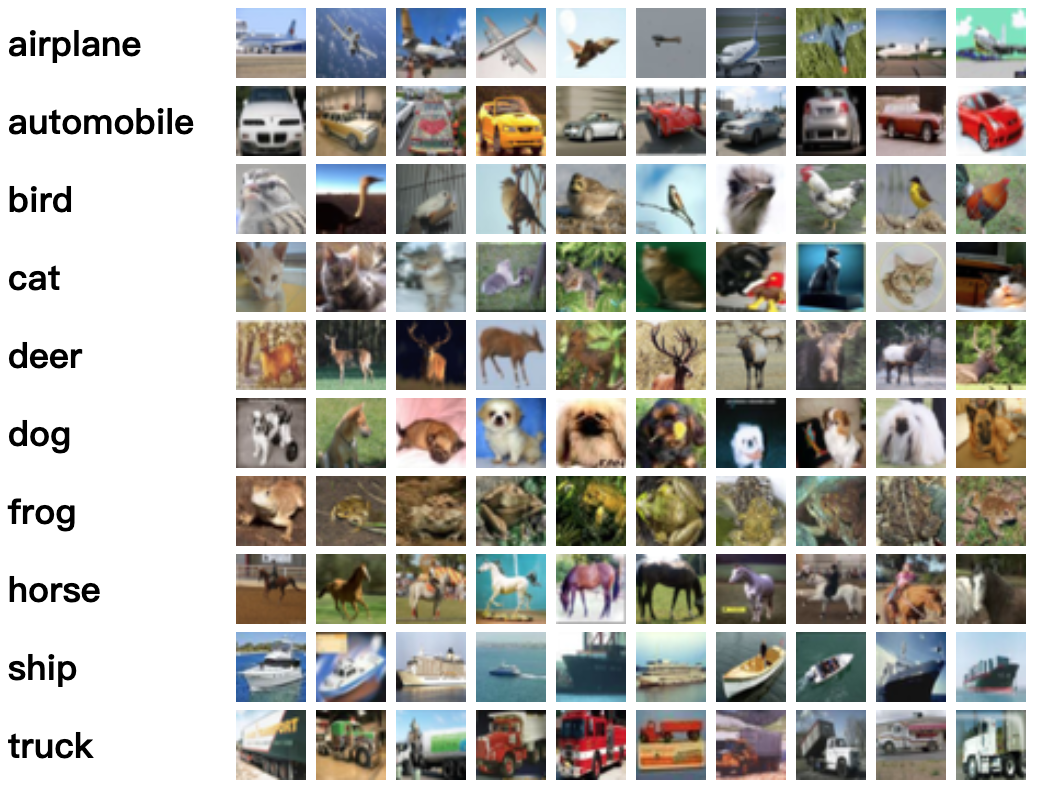
\includegraphics[width=0.68\linewidth]{../pic/CIFAR-10.png}
  \caption{CIFAR-10 数据集示意图。图像尺寸较小，但类别包含动物、交通工具等多种视觉模式。}
  \label{fig:cifar10_samples}
\end{figure}

\section{CIFAR-10 分类实验}

\subsection{实验路线概述}

第一部分的目标是尽可能降低 CIFAR-10 测试错误率，同时满足项目对网络组件、优化策略和可视化分析的要求。我的实验路线大致分为三个阶段：

\begin{enumerate}
  \item 建立基线模型。首先实现 classic CNN，随后训练 ResNet-110、DenseNet-BC、WideResNet 等更强基线，以获得模型容量、训练时间和泛化性能之间的参照。
  \item 设计改进模型。基于 DenseNet-BC 结构加入 SE channel attention、stochastic depth、Dropout、强数据增强、CutMix 和 EMA，形成 MyDenseNet 系列。
  \item 进行消融和最终复跑。在 \path{Ablation/} 中重新实现独立的训练、消融和可视化代码，使用 50 epoch 短预算比较容量、激活函数、损失函数和优化器，最后用消融推荐配置进行 300 epoch 完整训练。
\end{enumerate}

最终提交模型不是直接采用参数量最大的 SE-DenseNet-BC-190-40，而是采用消融后得到的 SE-DenseNet-BC-190-24。它在参数量大幅下降的同时取得更好的测试结果，因此更符合项目评分中对准确率、参数量、结构合理性和训练代价的综合要求。

\subsection{网络结构}

最终模型是一个面向 CIFAR-10 的 SE-DenseNet-BC。DenseNet 的核心思想是将同一 dense block 内所有先前层的输出拼接为当前层输入：
\[
x_l = H_l([x_0,x_1,\ldots,x_{l-1}]).
\]
这种 dense connection 可以增强特征复用，并改善梯度传播。相比普通残差网络，DenseNet 不是简单相加，而是在通道维度拼接特征，因此每一层都可以直接访问较浅层表示。

本实验采用 DenseNet-BC 变体。其中 B 表示 bottleneck：每个 dense layer 先使用 $1\times1$ 卷积压缩通道，再使用 $3\times3$ 卷积生成 $k$ 个新特征；C 表示 compression：transition layer 中使用 $1\times1$ 卷积将通道数乘以压缩率 $\theta$，随后使用平均池化降低空间分辨率。最终模型的主要结构如表~\ref{tab:final_architecture} 所示。

\begin{table}[H]
  \centering
  \caption{最终 SE-DenseNet-BC-190-24 的结构配置}
  \label{tab:final_architecture}
  \begin{tabular}{ll}
    \toprule
    项目 & 配置 \\
    \midrule
    模型 & SE-DenseNet-BC \\
    Depth & 190 \\
    Layers per dense block & 31 \\
    Growth rate & 24 \\
    Compression & 0.5 \\
    Activation & GELU \\
    SE reduction & 16 \\
    Stochastic depth rate & 0.2 \\
    Classifier hidden dim & 512 \\
    Classifier dropout & 0.2 \\
    Trainable parameters & 9,978,062 \\
    \bottomrule
  \end{tabular}
\end{table}

该模型满足项目对基础网络组件的要求。卷积部分由大量 \texttt{Conv2d}、BatchNorm 和 GELU 构成；transition layer 包含平均池化；分类器包含全连接层；同时模型还包含 Dropout、Dense connection、SE attention 和 stochastic depth 等额外组件。

SE attention 的作用是进行通道级重标定。对某一层输出特征 $U\in\mathbb{R}^{C\times H\times W}$，先通过全局平均池化得到通道描述，再经过两层小型 MLP 产生通道权重，最后对原特征逐通道缩放。这使模型可以自适应强调更有判别力的通道。Stochastic depth 则在训练时随机跳过部分层的残差式贡献，相当于对非常深的网络施加路径级正则化，有助于降低过拟合。

\subsection{训练策略}

最终模型使用较强的训练 recipe，配置见表~\ref{tab:final_training_recipe}。训练共 300 epoch，batch size 为 64，优化器为 SGD with momentum，学习率从 0.1 按 cosine schedule 衰减到 $10^{-5}$。损失函数为交叉熵加 label smoothing，平滑系数为 0.1。

\begin{table}[H]
  \centering
  \caption{最终模型训练配置}
  \label{tab:final_training_recipe}
  \begin{tabular}{ll}
    \toprule
    项目 & 设置 \\
    \midrule
    Epochs & 300 \\
    Batch size & 64 \\
    Optimizer & SGD + momentum 0.9 \\
    Initial learning rate & 0.1 \\
    Minimum learning rate & $10^{-5}$ \\
    Scheduler & Cosine annealing \\
    Weight decay & $10^{-4}$ \\
    Loss & CrossEntropy + label smoothing 0.1 \\
    Data augmentation & Random crop/flip + AutoAugment + Cutout \\
    Mix strategy & CutMix, $\alpha=1.0$ \\
    EMA decay & 0.999 \\
    Mixed precision & Enabled \\
    \bottomrule
  \end{tabular}
\end{table}

需要说明的是，最终训练日志中的 train accuracy 不能直接解释为干净训练集准确率。由于训练过程中使用 CutMix、强数据增强和 label smoothing，训练 batch 的标签与图像都经过混合和扰动，因此训练准确率会显著低于测试准确率。这并不表示模型欠拟合，而是强正则化训练配方下的正常现象。最终验证时使用干净测试集，并加载 EMA 权重。

\subsection{基线模型对比}

为判断最终模型是否真正带来改进，我训练或整理了多个 baseline。表~\ref{tab:baseline_comparison} 汇总了主要模型的最好测试准确率和错误率。

\begin{table}[H]
  \centering
  \caption{CIFAR-10 主要模型结果对比}
  \label{tab:baseline_comparison}
  \begin{tabular}{lccc}
    \toprule
    模型 & 目录 & Best test accuracy & Test error \\
    \midrule
    Classic CNN & \path{classic_CNN/} & $74.04\%$ & $25.96\%$ \\
    ResNet-110 & \path{classic_ResNet-110/} & $93.40\%$ & $6.60\%$ \\
    DenseNet-BC-100-24 & \path{classic_DenseNet/} & $96.42\%$ & $3.58\%$ \\
    WideResNet-28-10 & \path{classic_WideResNet/} & $96.63\%$ & $3.37\%$ \\
    SE-DenseNet-BC-190-40 & \path{my_DenseNet/} & $96.68\%$ & $3.32\%$ \\
    SE-StochasticDepth-WRN-40-10 & \path{my_final_CNN/} & $91.08\%$ & $8.92\%$ \\
    \textbf{Final SE-DenseNet-BC-190-24} & \path{Ablation/} & $\mathbf{97.15\%}$ & $\mathbf{2.85\%}$ \\
    \bottomrule
  \end{tabular}
\end{table}

可以看到，简单 CNN 只能达到约 $74\%$ 准确率；ResNet-110 将错误率降至 $6.60\%$；DenseNet-BC 和 WideResNet 进一步接近 $3.5\%$ 错误率。早期候选模型 SE-DenseNet-BC-190-40 的错误率为 $3.32\%$，已经强于这些 baseline，但其参数量约 26.76M。最终的 SE-DenseNet-BC-190-24 通过容量消融和激活函数选择，将参数量降至约 9.98M，同时把错误率进一步降到 $2.85\%$。

这说明最终提升并不只是来自堆叠更多参数，而是来自更合适的容量、激活函数和训练策略组合。另一个尝试 \path{my_final_CNN/} 中的 SE-StochasticDepth-WRN-40-10 表现不佳，说明强正则和复杂结构并不必然带来更高精度；模型结构与训练 recipe 的匹配更关键。

\subsection{消融实验}

项目要求尝试不同滤波器数量、不同损失函数、不同激活函数和不同优化器。为此，我在 \path{Ablation/} 中实现了自动化消融实验。消融实验统一使用 50 epoch 短预算，目的是比较不同设计在早期训练阶段的收敛趋势和泛化潜力。最终结果仍以 300 epoch 完整复跑为准。

\begin{table}[H]
  \centering
  \caption{50 epoch 消融实验结果}
  \label{tab:ablation_results}
  \begin{tabular}{llcc}
    \toprule
    组别 & 实验 & Best test accuracy & 参数量 \\
    \midrule
    Baseline & D190-K40 + SiLU + CE + SGD & $91.13\%$ & 26,763,454 \\
    Capacity & Growth rate 32 & $91.63\%$ & 17,357,022 \\
    Capacity & Growth rate 24 & $91.64\%$ & 9,978,062 \\
    Activation & ReLU & $92.99\%$ & 26,763,454 \\
    Activation & GELU & $\mathbf{93.13\%}$ & 26,763,454 \\
    Loss & Focal Loss & $89.35\%$ & 26,763,454 \\
    Optimizer & AdamW & $90.53\%$ & 26,763,454 \\
    Optimizer & RMSprop & $10.00\%$ & 26,763,454 \\
    \bottomrule
  \end{tabular}
\end{table}

消融实验有几个重要结论。

第一，减小 growth rate 反而提升了短训练预算下的测试准确率。默认 K40 模型参数量较大，50 epoch 时达到 $91.13\%$；K32 和 K24 分别达到 $91.63\%$ 与 $91.64\%$。这说明在当前强增强和短训练预算下，更小的容量并没有限制泛化，反而减少了过拟合和优化负担。由于 K24 参数量只有 K40 的约 $37.3\%$，最终模型采用 K24。

第二，GELU 优于 SiLU 和 ReLU。GELU 在消融中达到 $93.13\%$，略高于 ReLU 的 $92.99\%$，明显高于默认 SiLU 的 $91.13\%$。GELU 的平滑非线性可能更适合深层 DenseNet 中的特征传递，因此最终配置采用 GELU。

第三，Focal Loss 并未带来收益。CIFAR-10 是相对均衡的数据集，每类样本数相同；Focal Loss 更适合类别不平衡或难样本极端重要的场景。在本实验中，它使准确率下降到 $89.35\%$。因此最终仍使用 CrossEntropy + label smoothing。

第四，优化器选择非常关键。AdamW 在该配方下低于 SGD，RMSprop 则几乎完全失败，只达到随机猜测水平。这说明对于经过长期验证的 CIFAR-10 DenseNet 训练，SGD with momentum 配合 cosine schedule 仍然是更稳定的选择。

\begin{figure}[H]
  \centering
  \begin{subfigure}{0.48\linewidth}
    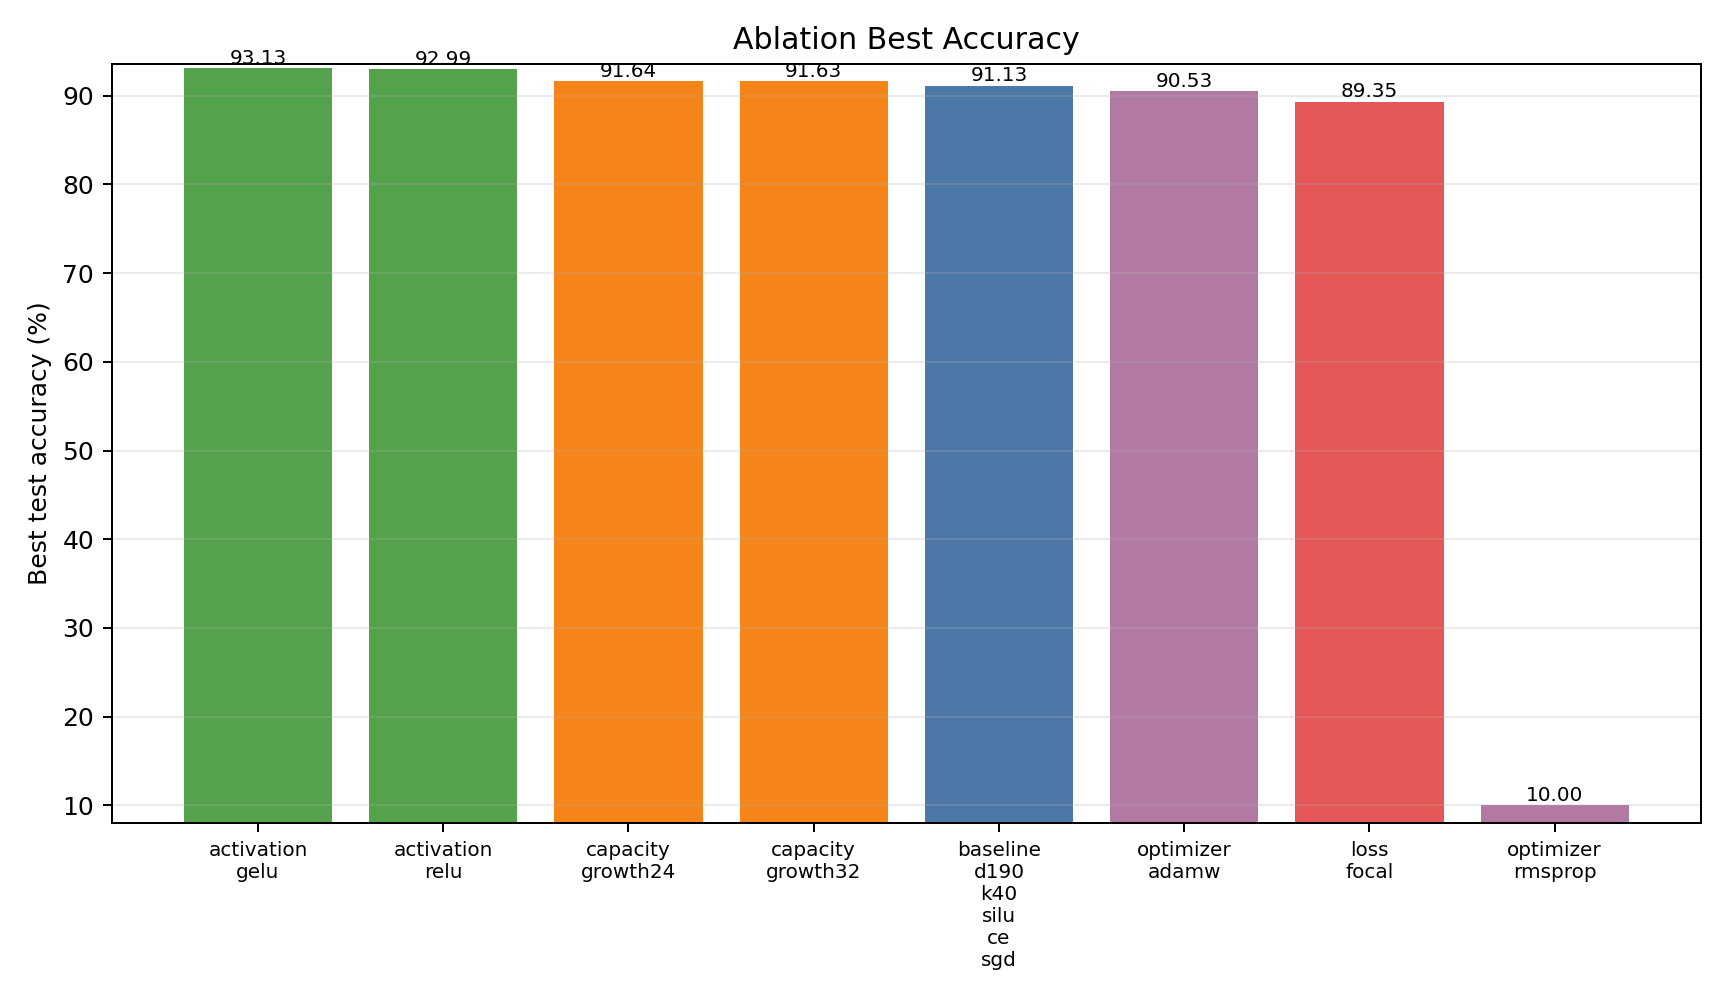
\includegraphics[width=\linewidth]{../Ablation/results/ablation/figures/ablation_best_accuracy.png}
    \caption{各消融实验最佳准确率}
  \end{subfigure}
  \hfill
  \begin{subfigure}{0.48\linewidth}
    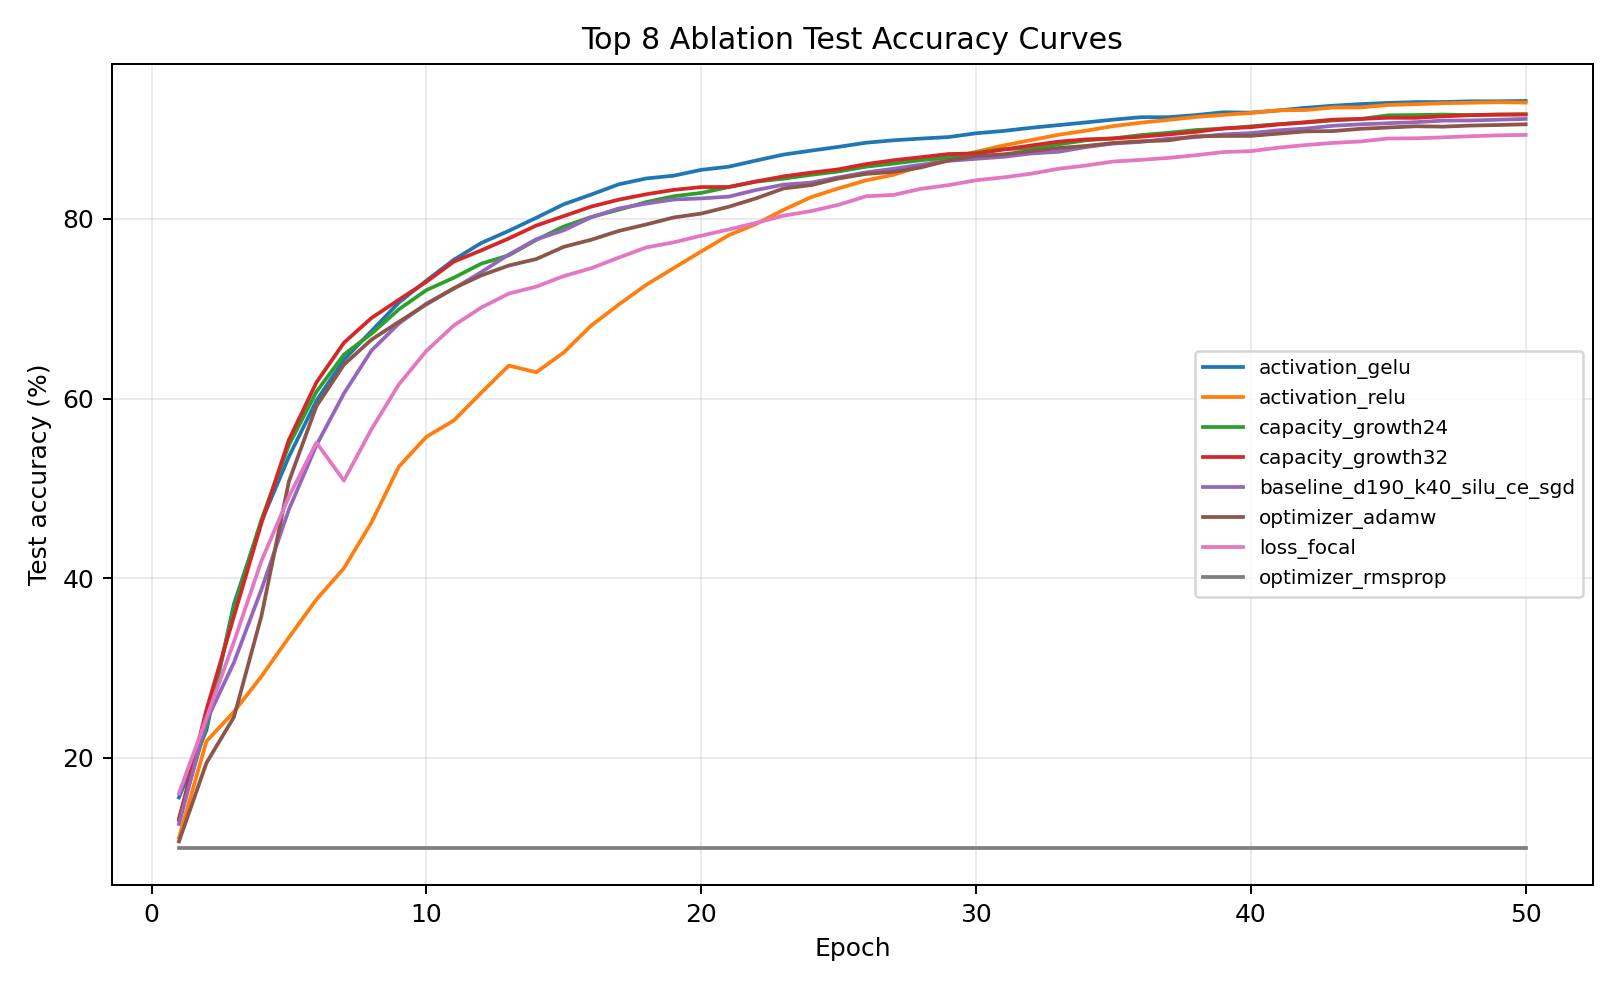
\includegraphics[width=\linewidth]{../Ablation/results/ablation/figures/ablation_learning_curves.png}
    \caption{消融实验学习曲线}
  \end{subfigure}
  \caption{第一部分 50 epoch 消融实验可视化。消融实验用于选择最终复跑配置，而不是直接代表最终模型精度。}
  \label{fig:ablation_visuals}
\end{figure}

\subsection{最终模型结果}

根据消融结果，最终模型采用 growth rate 24 和 GELU，并保持 CrossEntropy、label smoothing、SGD、CutMix、AutoAugment、Cutout、stochastic depth 与 EMA。完整训练 300 epoch 后，结果如表~\ref{tab:final_result} 所示。

\begin{table}[H]
  \centering
  \caption{最终模型在 CIFAR-10 测试集上的结果}
  \label{tab:final_result}
  \begin{tabular}{lc}
    \toprule
    指标 & 数值 \\
    \midrule
    Best epoch & 284 \\
    Best test accuracy & $\mathbf{97.15\%}$ \\
    Best test error & $\mathbf{2.85\%}$ \\
    Best test loss & 0.5846 \\
    Final epoch & 300 \\
    Final test accuracy & $97.13\%$ \\
    Final test loss & 0.5838 \\
    Correct / Total & 9715 / 10000 \\
    \bottomrule
  \end{tabular}
\end{table}

我还编写了 \texttt{quick\_check.py} 用于独立复核最终结果。该脚本读取最终配置和 \texttt{best.pt}，默认加载 EMA 权重，并在完整 CIFAR-10 test set 上评估。运行结果为：
\[
\mathrm{Accuracy}=97.15\%,\qquad
\mathrm{Error}=2.85\%.
\]
这与训练目录中的 \texttt{summary.json} 完全一致，说明最终模型权重、配置和评估流程是一致的。

\begin{figure}[H]
  \centering
  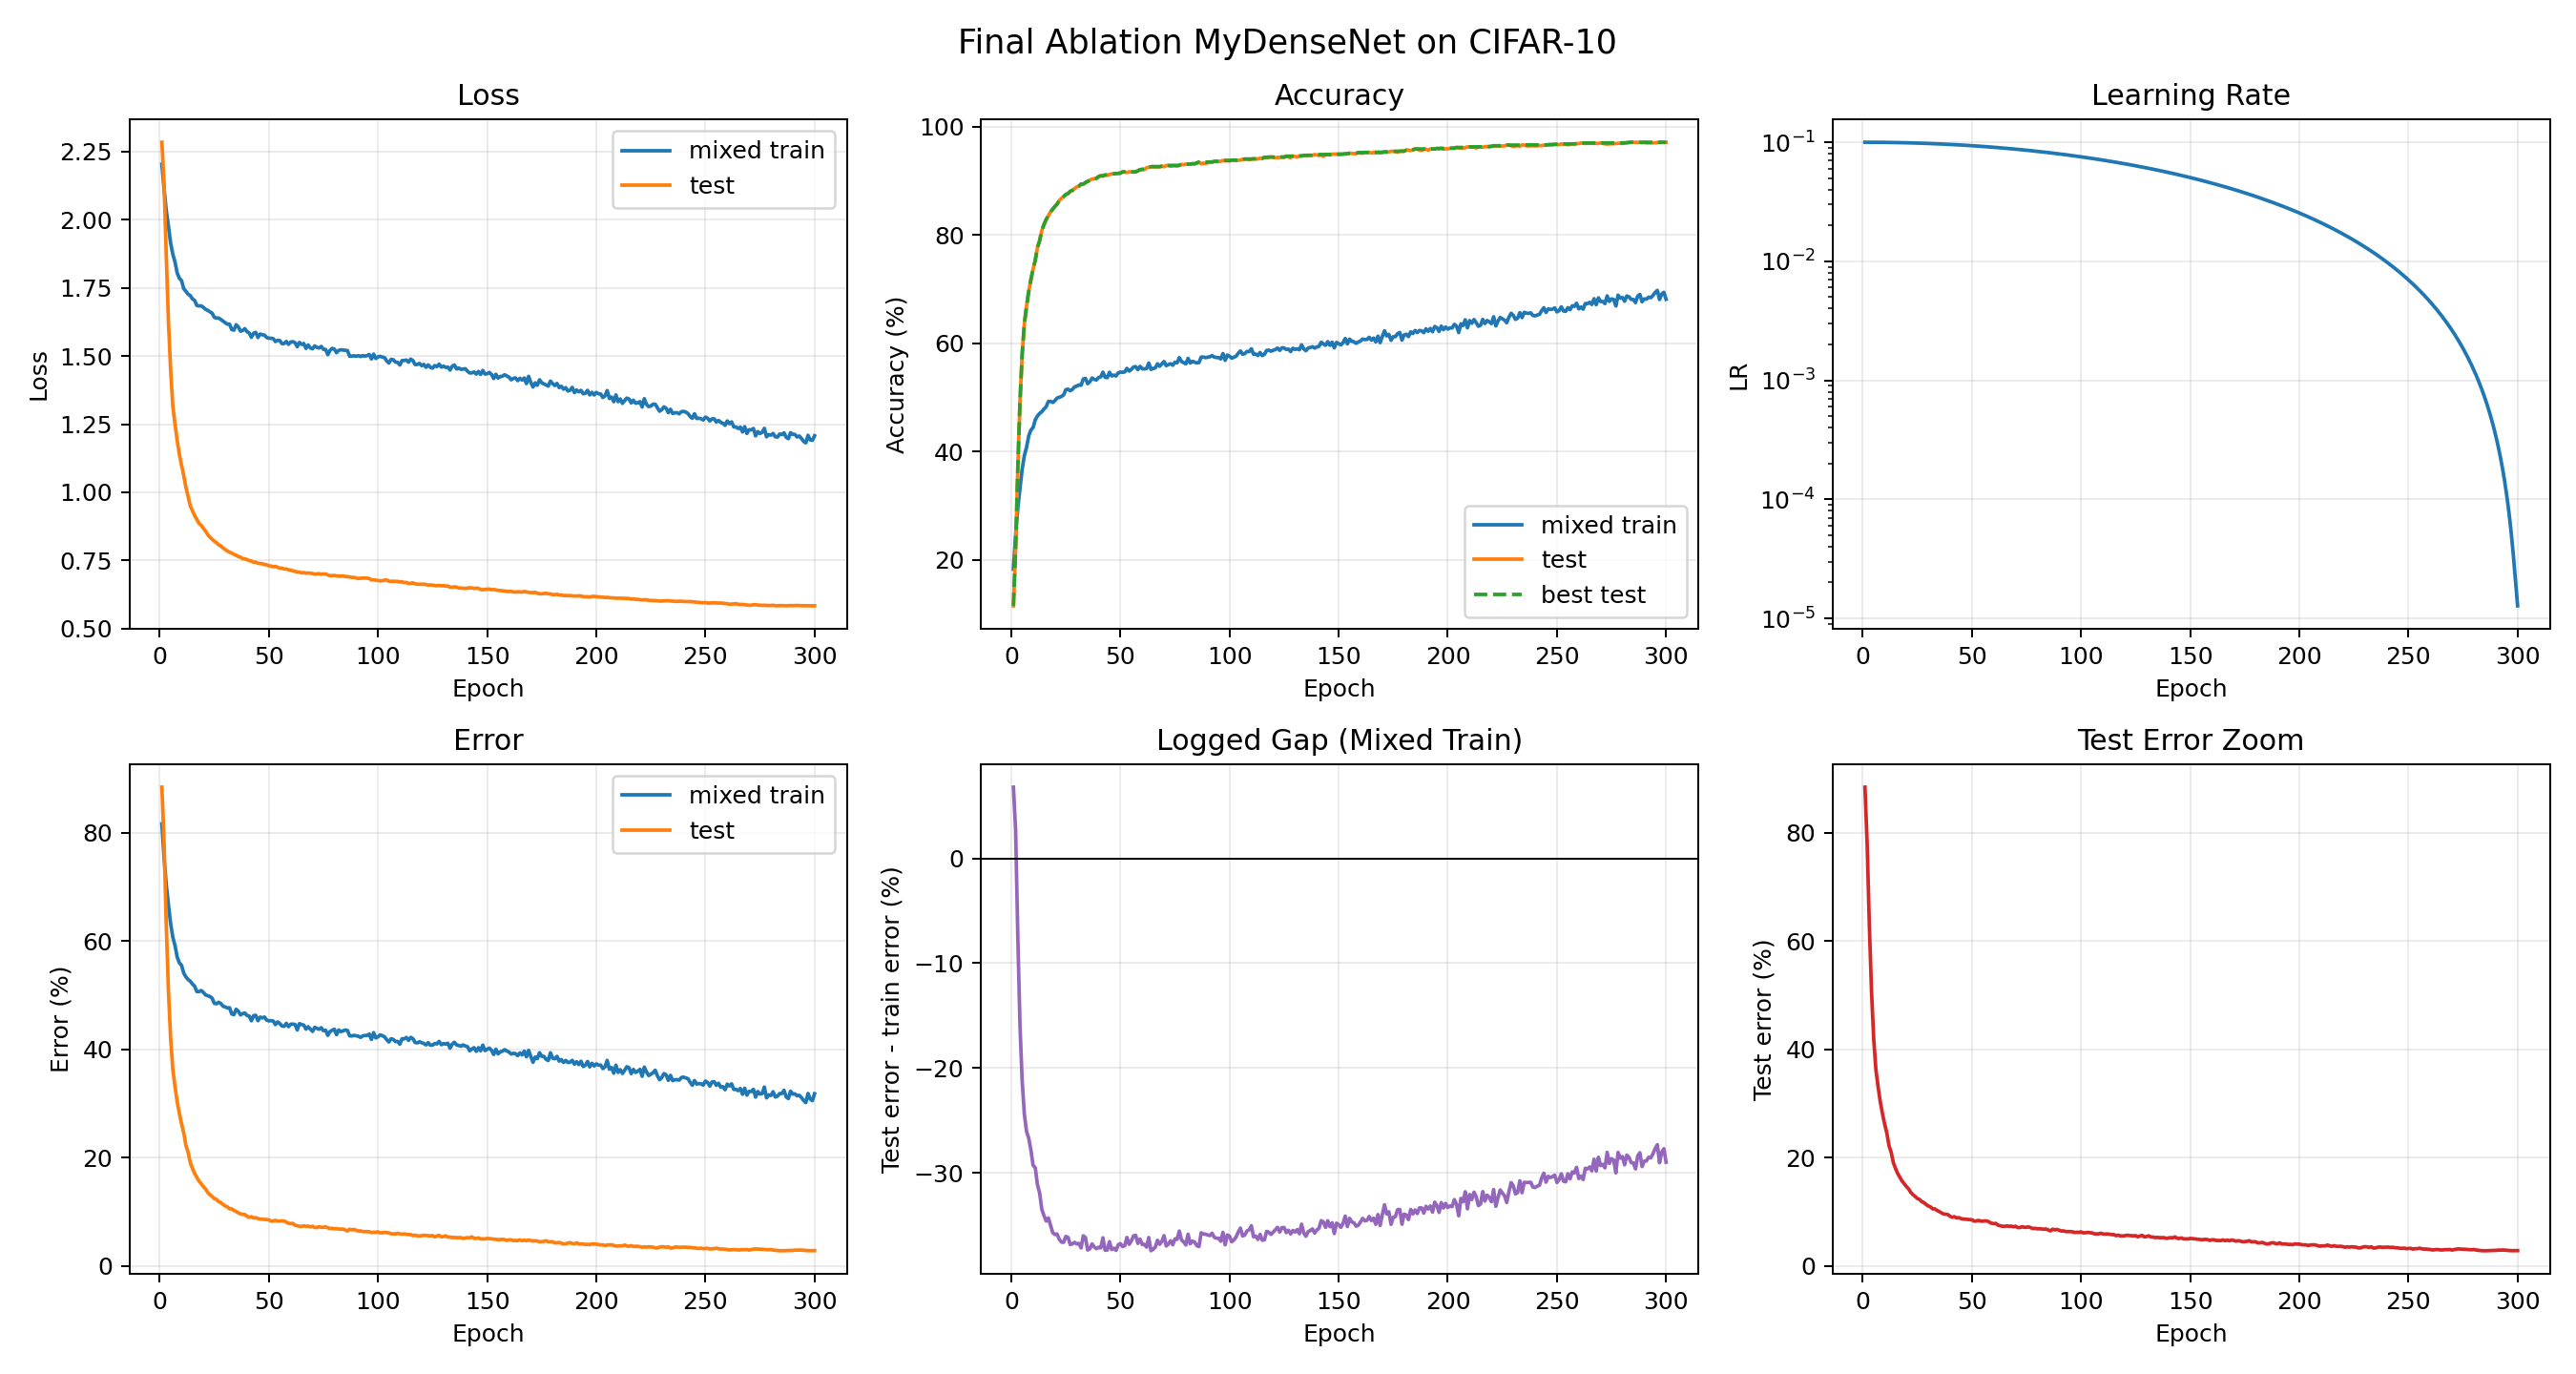
\includegraphics[width=0.9\linewidth]{../Ablation/results/final/best_from_ablation/curves.png}
  \caption{最终 SE-DenseNet-BC-190-24 的训练曲线。由于 CutMix 和强增强的存在，训练准确率不应直接与干净测试准确率比较。}
  \label{fig:final_curves}
\end{figure}

\subsection{最终模型可视化与解释}

为了满足项目对模型洞察的要求，我对最终模型进行了多种可视化分析，包括混淆矩阵、逐类准确率、置信度分布、误分类样例、第一层卷积核、Grad-CAM 和局部 loss landscape。

\begin{figure}[H]
  \centering
  \begin{subfigure}{0.48\linewidth}
    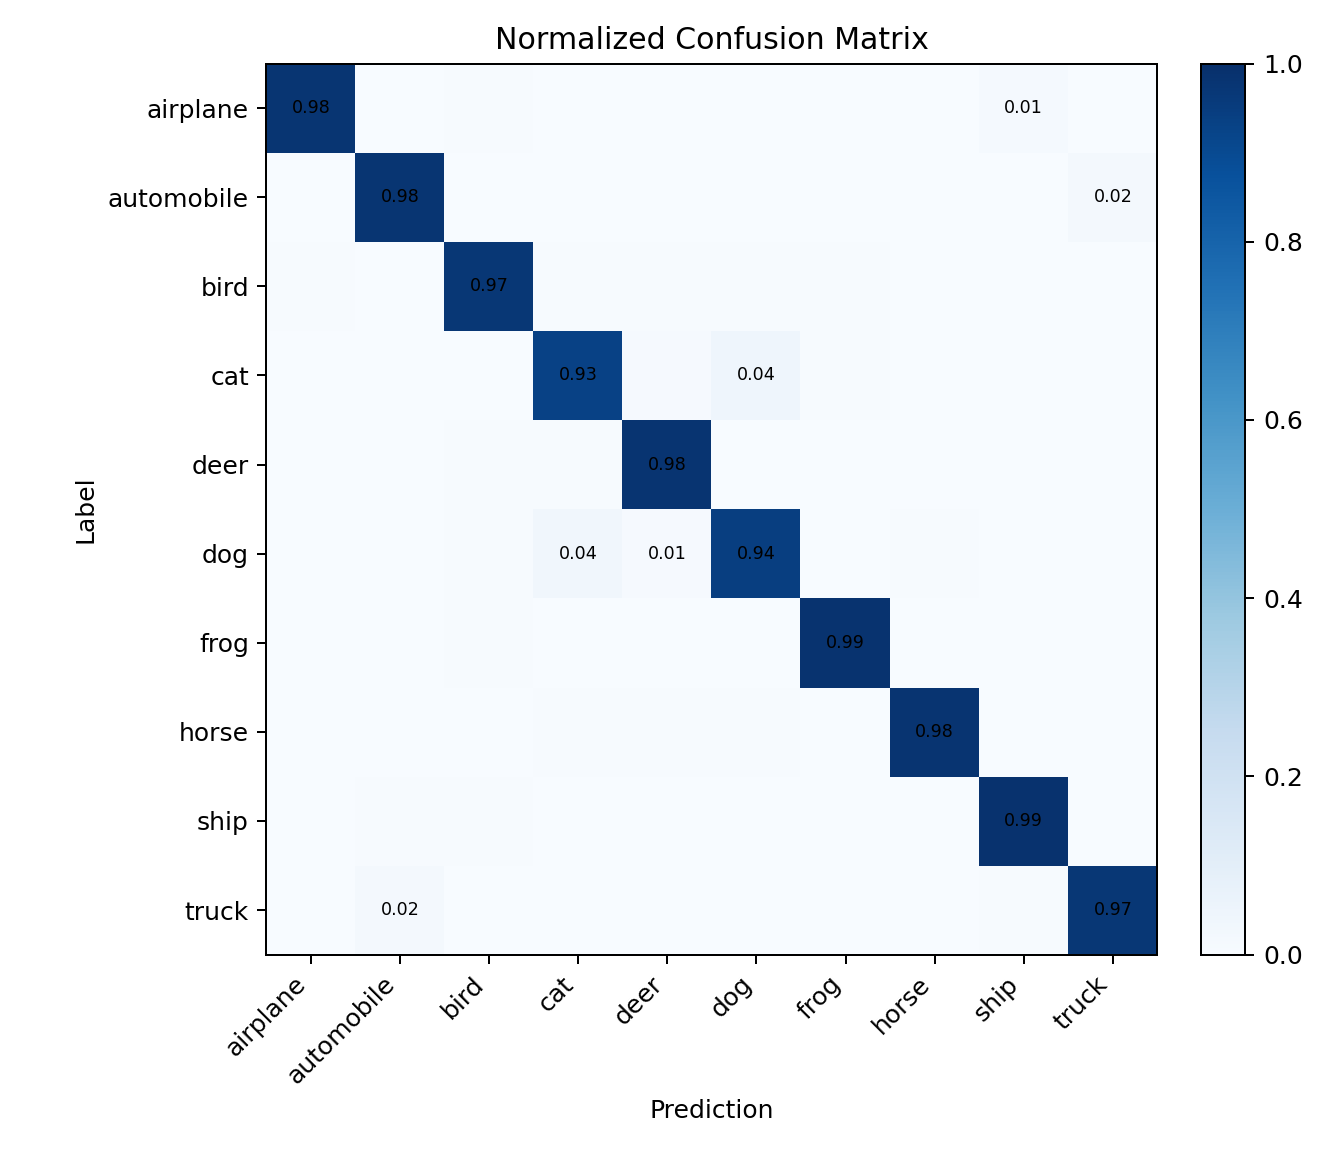
\includegraphics[width=\linewidth]{../Ablation/results/final/best_from_ablation/visualizations/confusion_matrix.png}
    \caption{混淆矩阵}
  \end{subfigure}
  \hfill
  \begin{subfigure}{0.48\linewidth}
    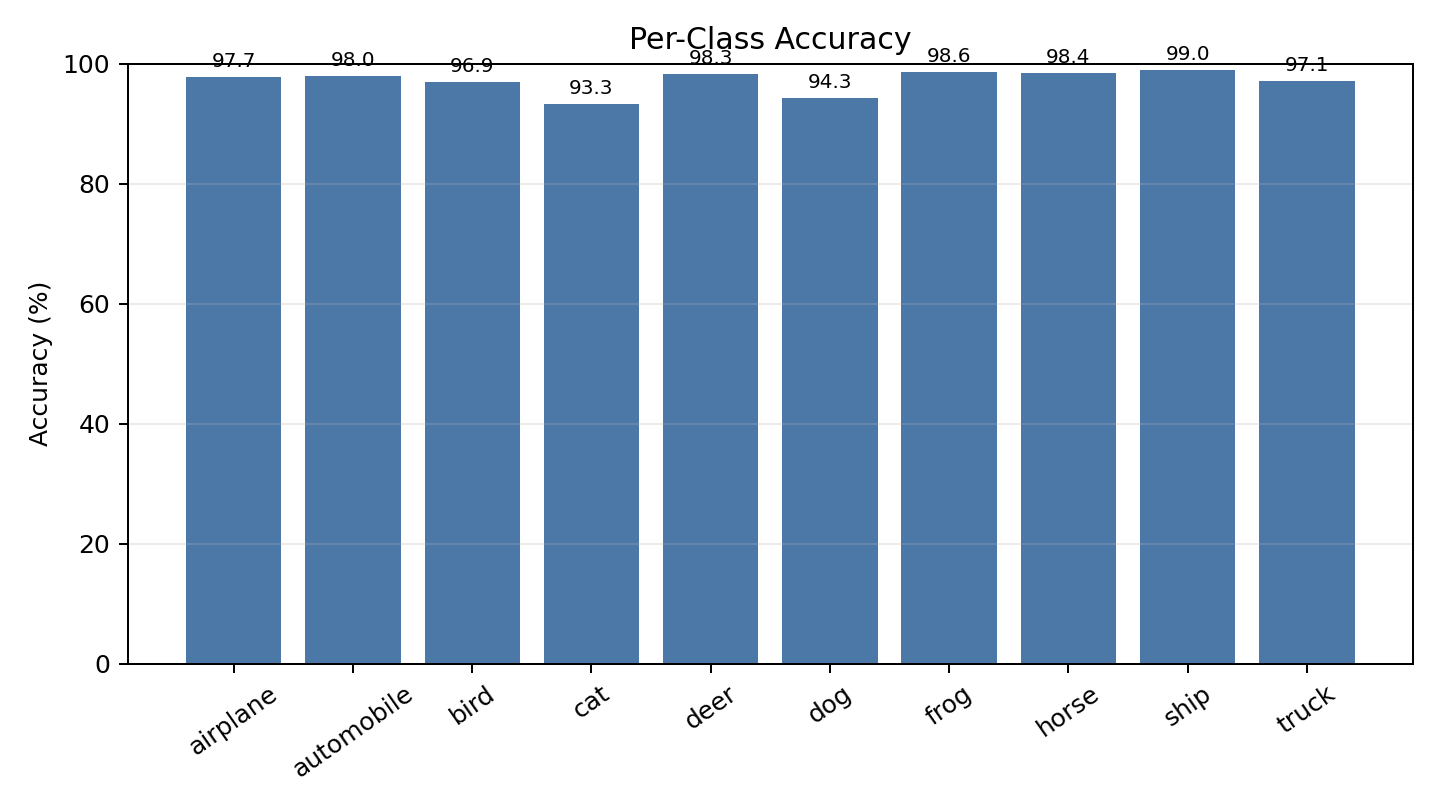
\includegraphics[width=\linewidth]{../Ablation/results/final/best_from_ablation/visualizations/per_class_accuracy.png}
    \caption{逐类准确率}
  \end{subfigure}
  \caption{最终模型分类结果可视化。整体错误率较低，主要混淆集中在视觉上相近的类别之间。}
  \label{fig:final_confusion_per_class}
\end{figure}

混淆矩阵说明最终模型在多数类别上具有稳定判别能力。逐类准确率图显示 ship、frog、horse、deer 等类别表现较强，而 cat 和 dog 这类局部纹理相似、姿态变化较大的类别仍是相对更难的部分。这与 CIFAR-10 上常见的错误模式一致。

\begin{figure}[H]
  \centering
  \begin{subfigure}{0.48\linewidth}
    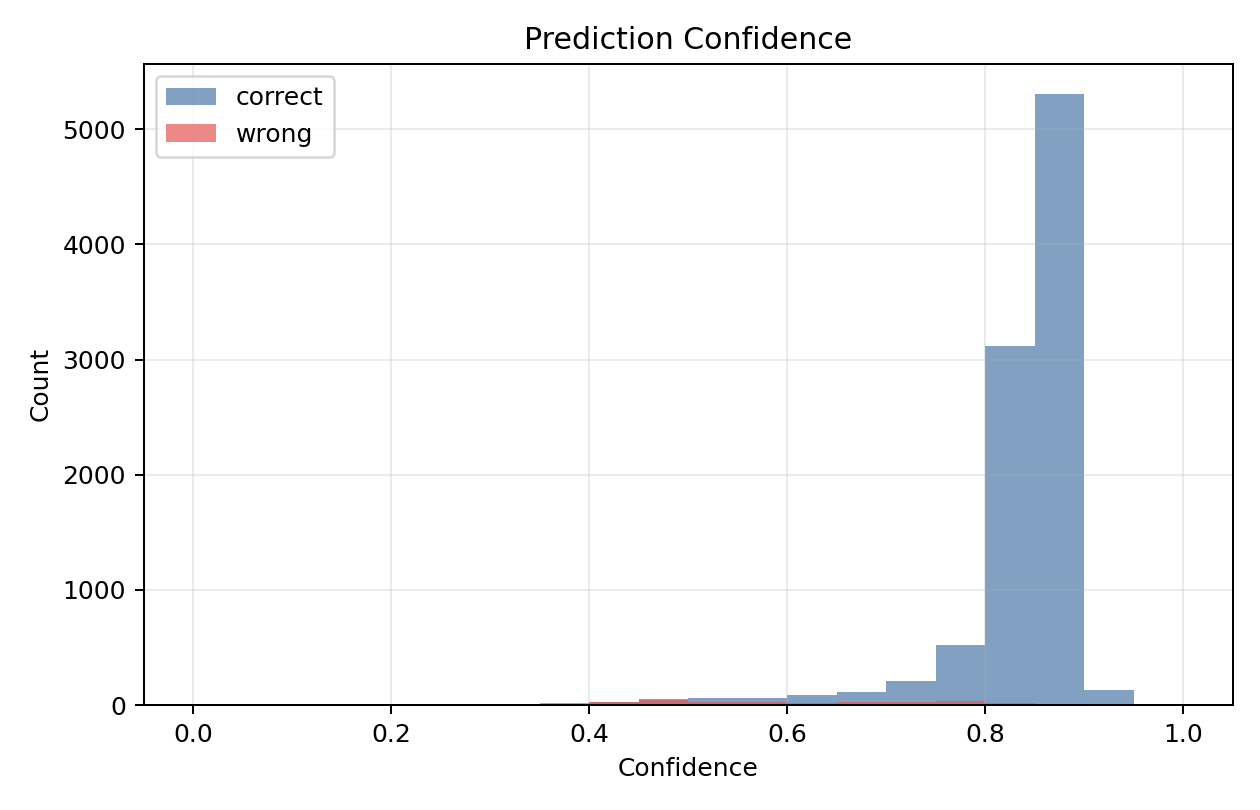
\includegraphics[width=\linewidth]{../Ablation/results/final/best_from_ablation/visualizations/confidence_histogram.png}
    \caption{预测置信度分布}
  \end{subfigure}
  \hfill
  \begin{subfigure}{0.48\linewidth}
    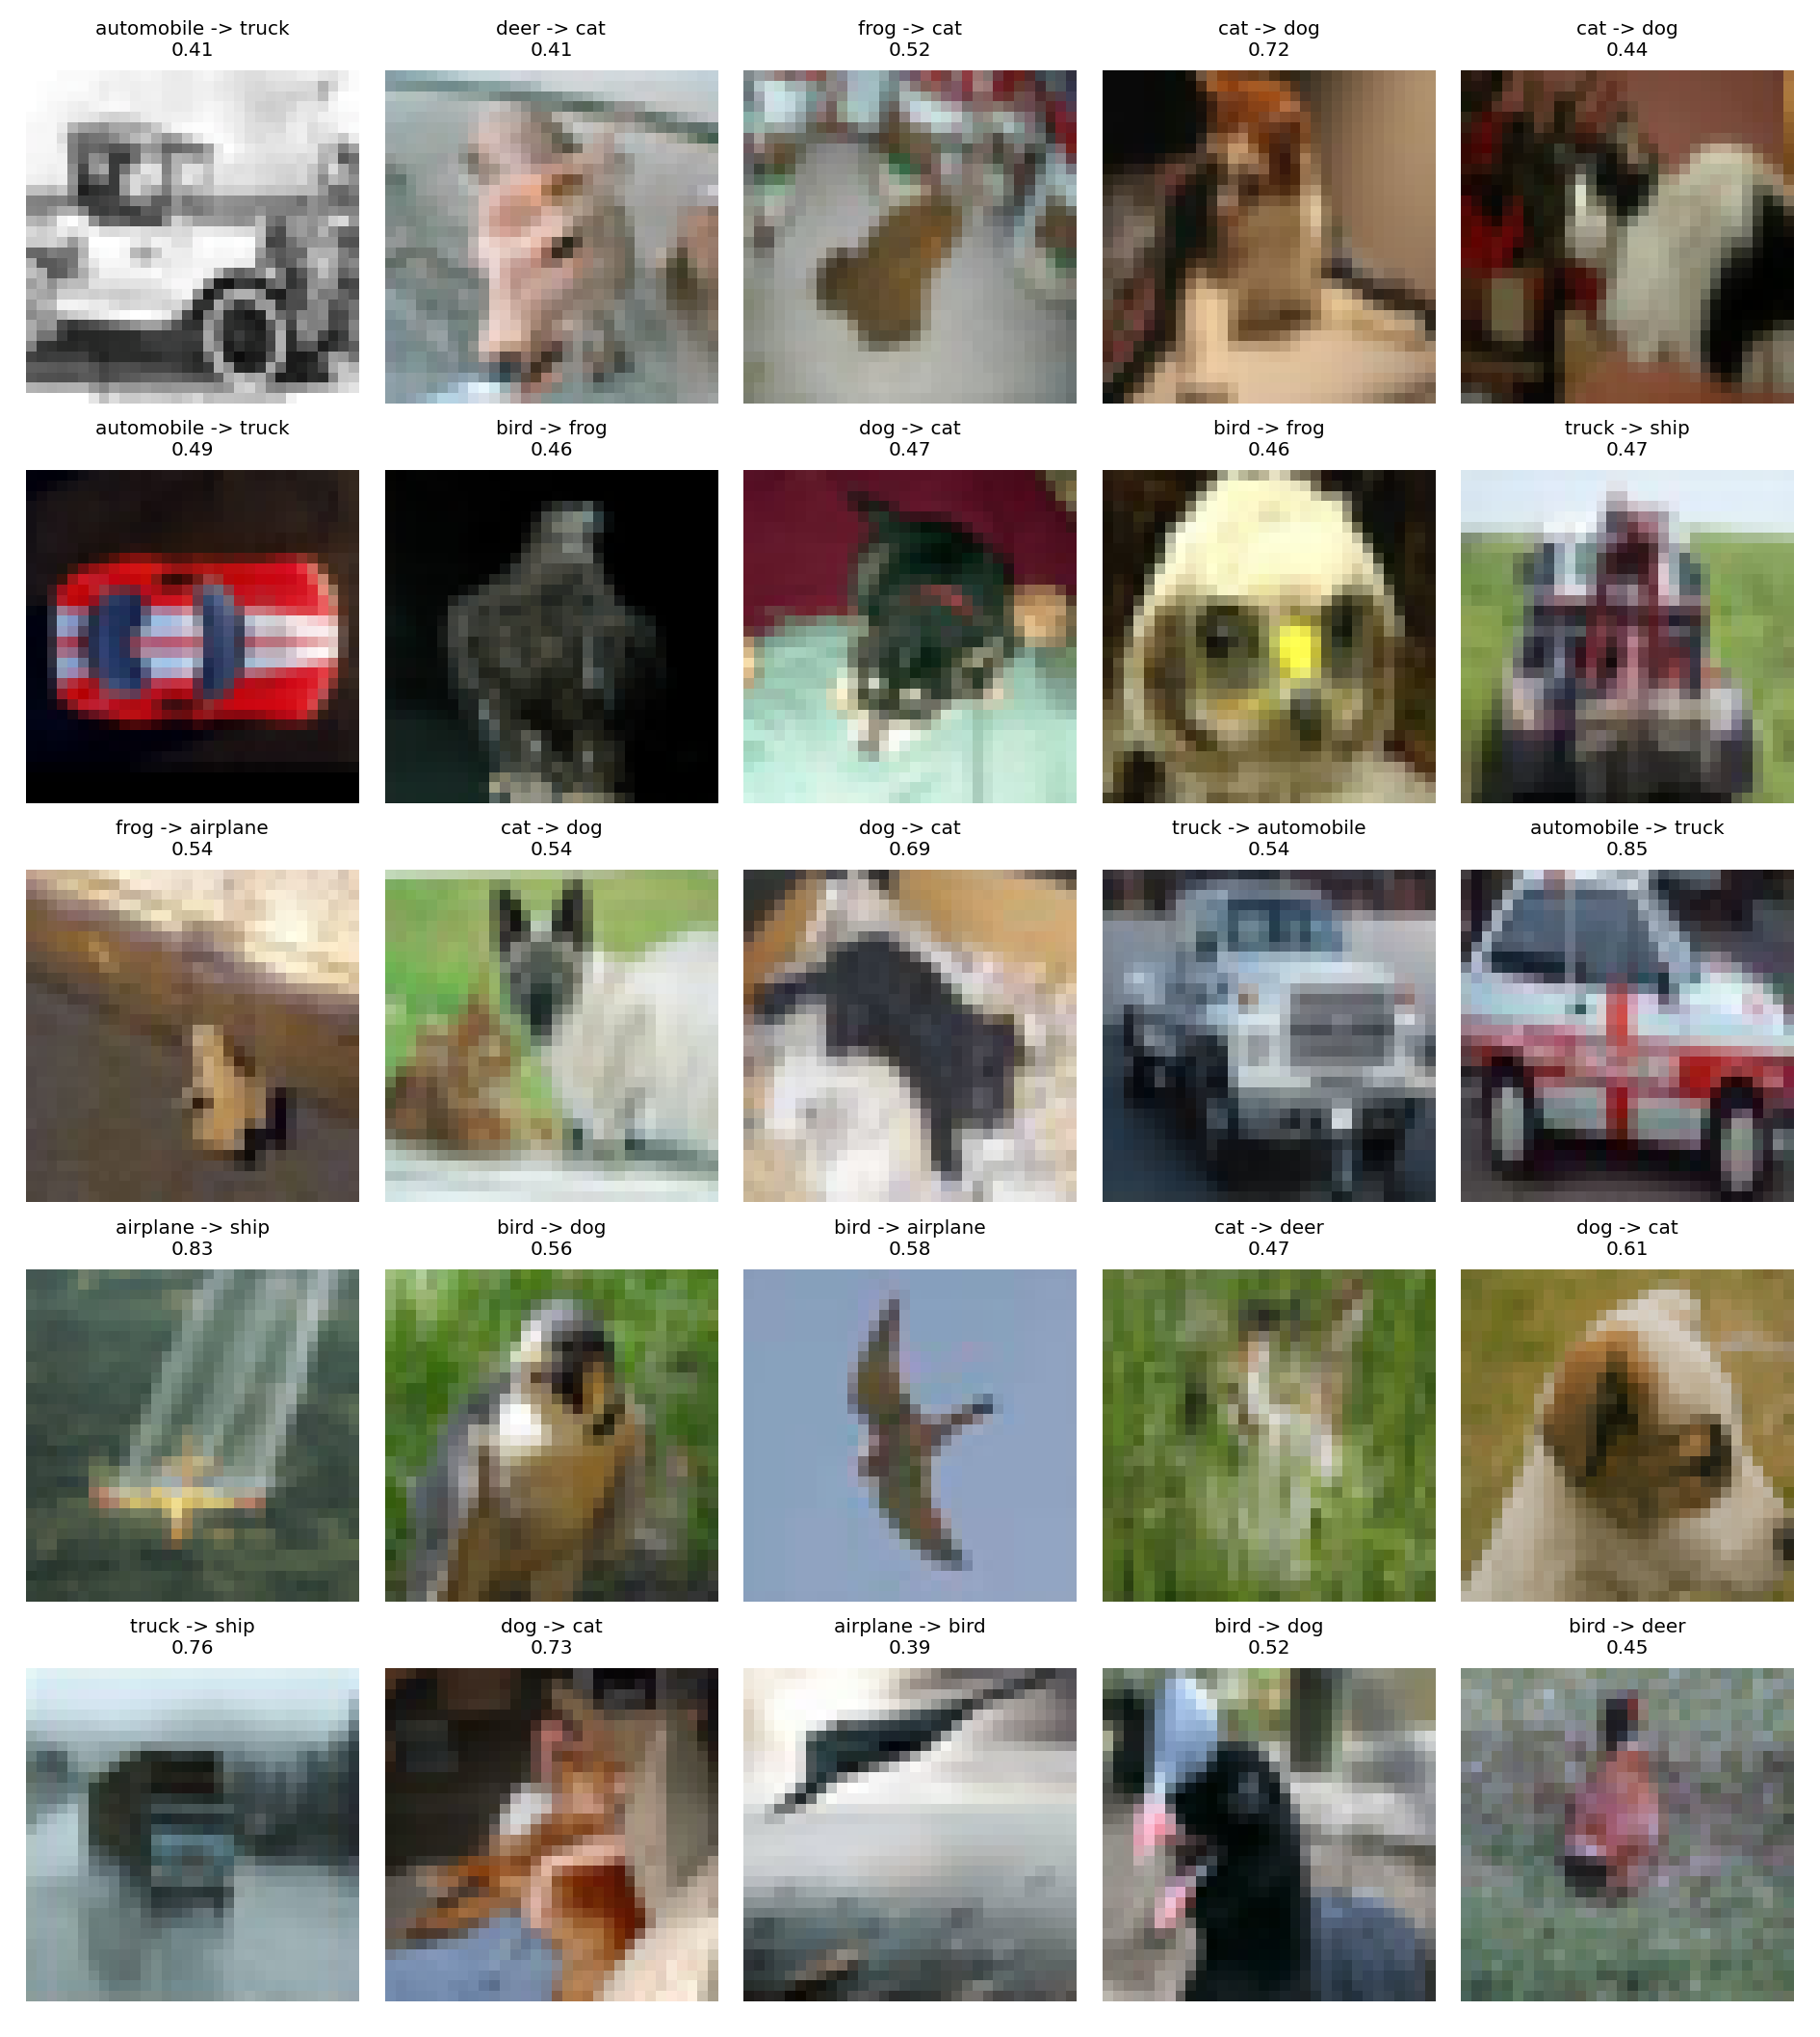
\includegraphics[width=\linewidth]{../Ablation/results/final/best_from_ablation/visualizations/misclassified_examples.png}
    \caption{误分类样例}
  \end{subfigure}
  \caption{置信度和错误样例分析。正确样本通常具有较高置信度，误分类样本多来自目标小、背景复杂或类别外观相近的图像。}
  \label{fig:confidence_misclassified}
\end{figure}

置信度分布用于观察模型是否在多数样本上形成明确判断。误分类样例则提供了更具体的失败模式：部分样本分辨率低、主体区域小，或目标形态与另一类高度接近，因此即使模型整体准确率较高，仍会出现合理但错误的预测。

\begin{figure}[H]
  \centering
  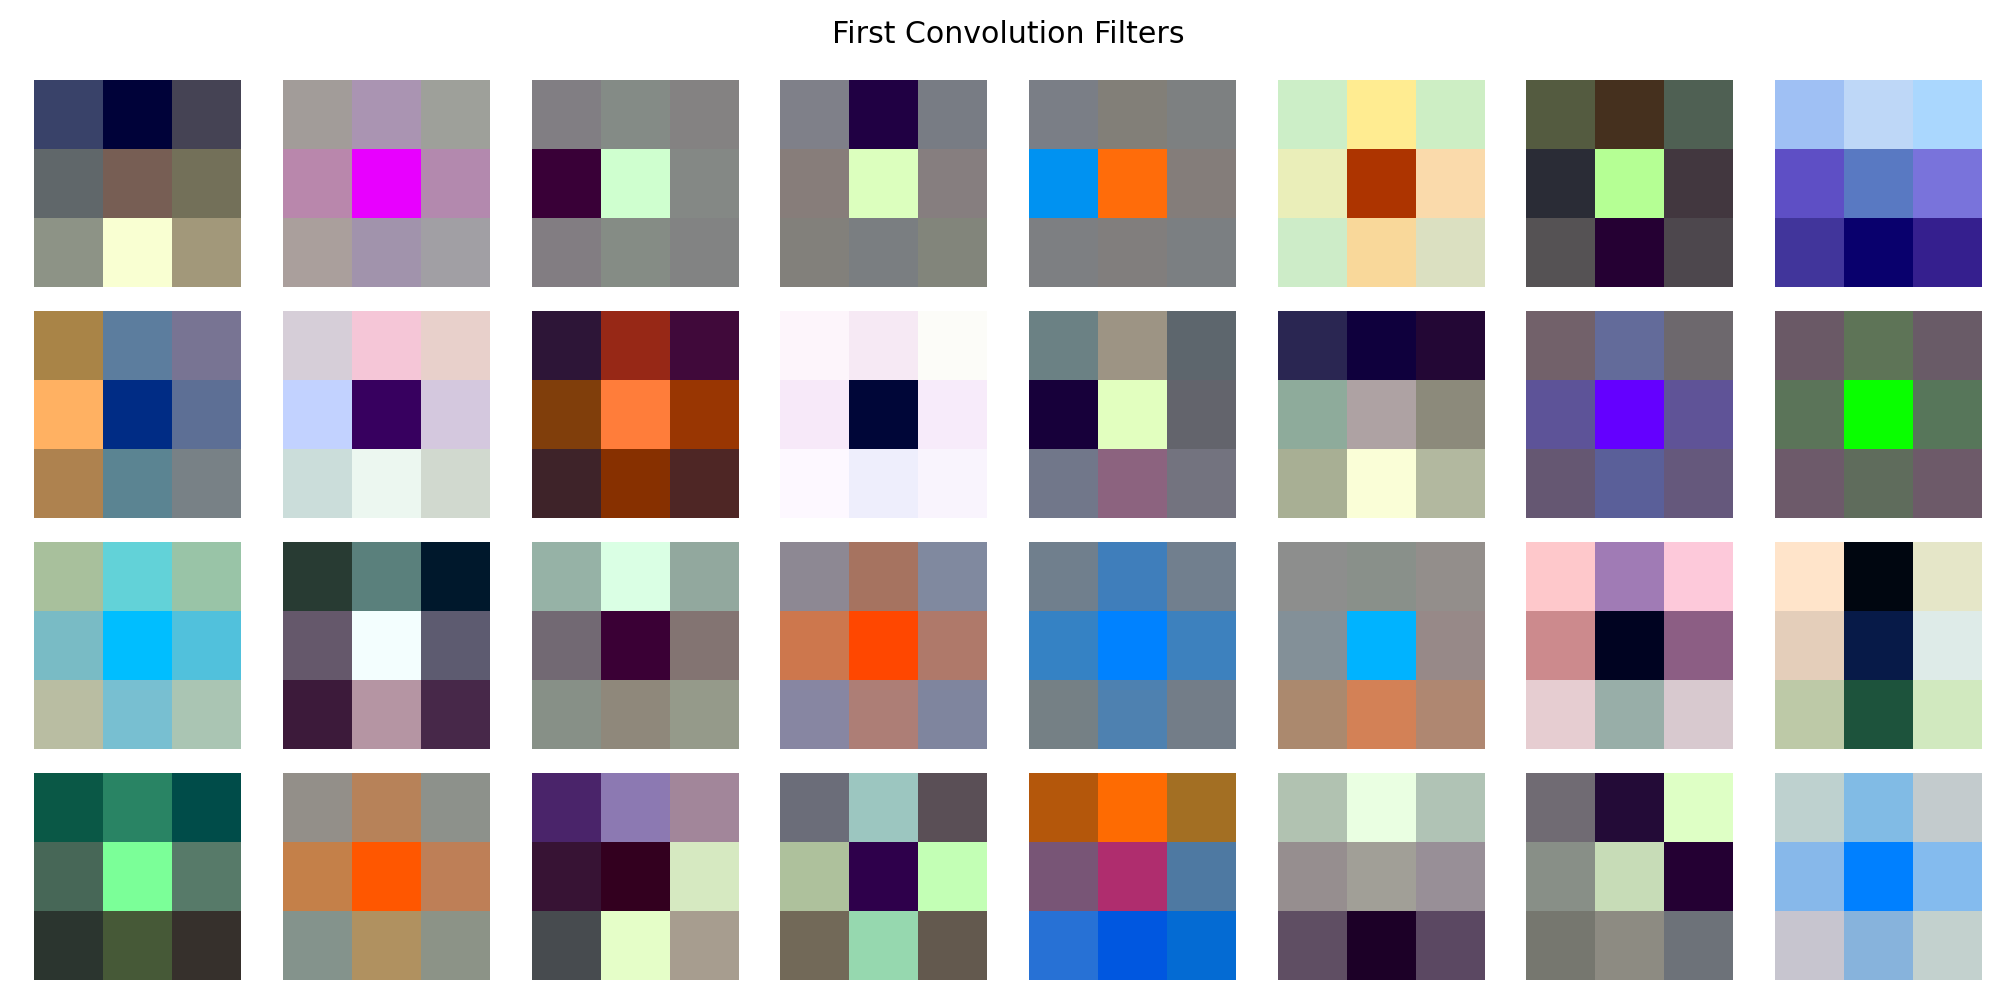
\includegraphics[width=0.58\linewidth]{../Ablation/results/final/best_from_ablation/visualizations/first_conv_filters.png}
  \caption{最终模型第一层卷积核。浅层滤波器主要学习颜色对比、边缘和局部纹理等基础视觉模式。}
  \label{fig:first_conv_filters}
\end{figure}

\begin{figure}[H]
  \centering
  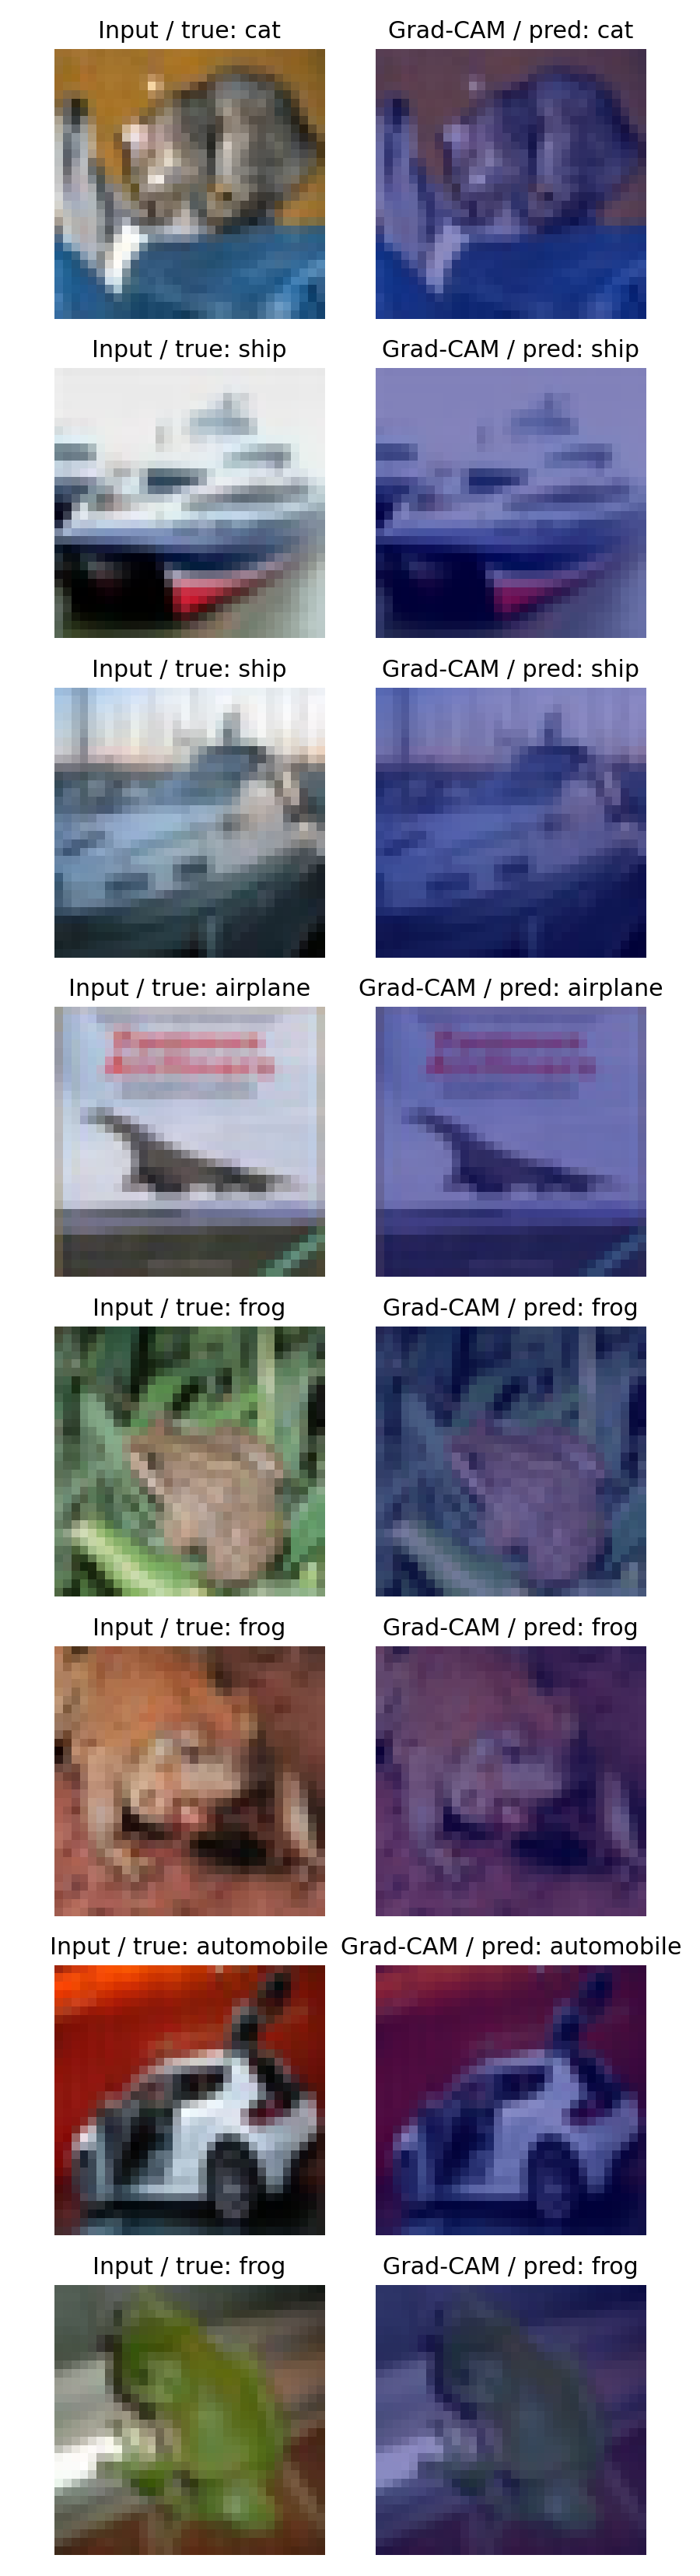
\includegraphics[width=0.82\linewidth,height=0.64\textheight,keepaspectratio]{../Ablation/results/final/best_from_ablation/visualizations/gradcam_examples.png}
  \caption{最终模型 Grad-CAM 示例。高响应区域通常覆盖目标主体，说明模型预测主要依赖图像中的语义目标，而不是完全依赖背景。}
  \label{fig:gradcam_examples}
\end{figure}

第一层卷积核展示了模型对颜色对比、边缘和局部纹理的基础检测。Grad-CAM 则进一步说明最终分类决策通常集中在图像中的目标主体区域。这一点对验证模型是否学习到合理视觉线索非常重要。

\begin{figure}[H]
  \centering
  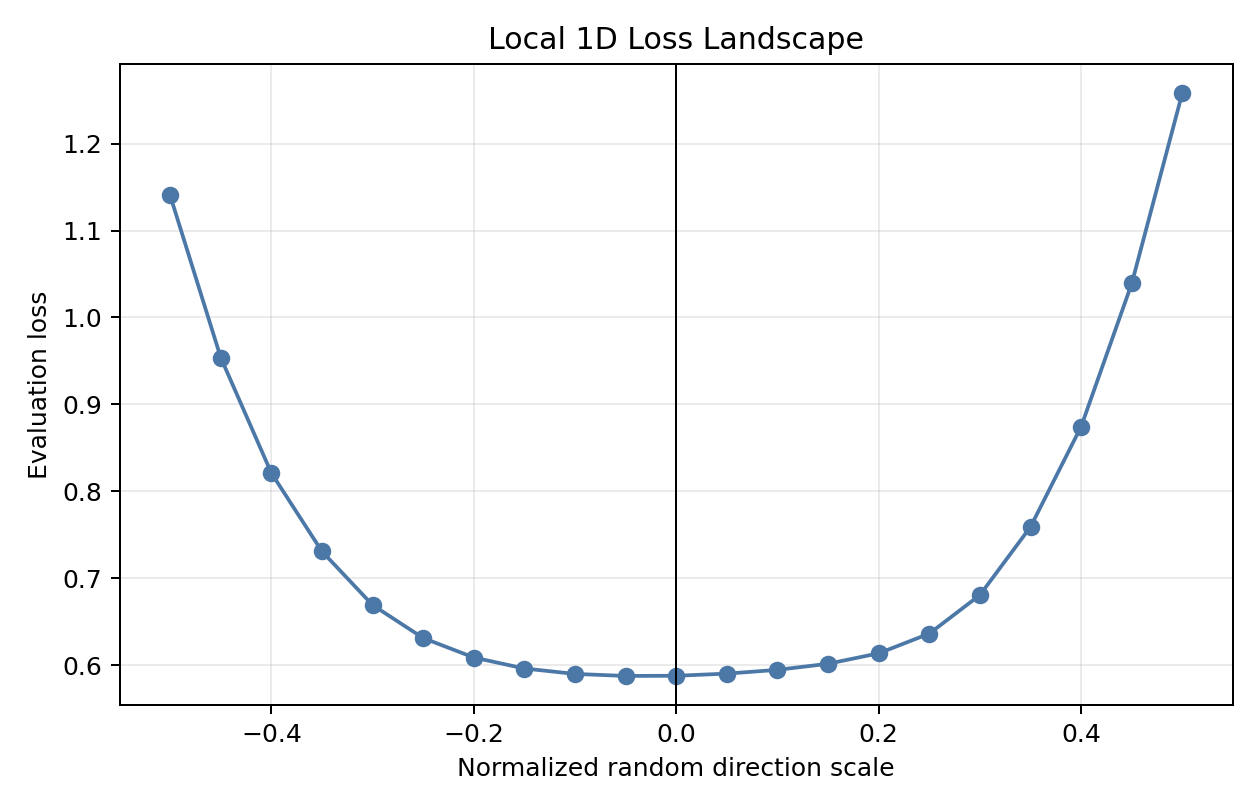
\includegraphics[width=0.72\linewidth]{../Ablation/results/final/best_from_ablation/loss_landscape/loss_landscape.png}
  \caption{最终模型附近的一维局部 loss landscape。该图不是全局损失面，只用于观察 checkpoint 附近随机方向上的局部稳定性。}
  \label{fig:final_loss_landscape}
\end{figure}

局部 loss landscape 显示，在最终 checkpoint 附近沿随机方向扰动参数时，loss 变化整体平滑。这与最终模型较好的泛化表现一致。不过，高维模型的 loss landscape 很难通过单个方向完整刻画，因此该图主要作为直观补充，不能单独作为严格结论。

\section{Batch Normalization 实验}

\subsection{BN 实验目标}

第二部分的目标是研究 Batch Normalization 对训练过程的影响。根据项目说明，需要先比较 VGG-A 与 VGG-A-BN 的性能，再分析 BN 如何帮助优化。为此，我在 \path{Batch_Normalization/} 中实现了基础实验，在 \path{Batch_Normalization/Enhanced/} 中补充学习率敏感性和梯度预测性实验，并在 \path{Batch_Normalization/Visual/} 中生成报告级可视化图。

BN 对卷积特征的归一化可写为：
\[
O_{b,c,x,y}
=
\gamma_c
\frac{I_{b,c,x,y}-\mu_c}{\sqrt{\sigma_c^2+\epsilon}}
+\beta_c,
\]
其中
\[
\mu_c=\frac{1}{|\mathcal B|}\sum_{b,x,y} I_{b,c,x,y},
\qquad
\sigma_c^2=\frac{1}{|\mathcal B|}\sum_{b,x,y}(I_{b,c,x,y}-\mu_c)^2.
\]
也就是说，BN 对同一通道内所有 batch 样本和空间位置共同统计均值与方差，然后做标准化和可学习的仿射变换。训练阶段使用当前 mini-batch 统计量并维护 running statistics；测试阶段使用累计的 running mean 和 running variance。

\subsection{VGG-A 与 VGG-A-BN 设置}

基础网络采用适配 CIFAR-10 的 VGG-A。输入为 $32\times32\times3$ 图像，卷积通道配置为：
\[
64,\ M,\ 128,\ M,\ 256,\ 256,\ M,\ 512,\ 512,\ M,\ 512,\ 512,\ M,
\]
其中 $M$ 表示 $2\times2$ max pooling。卷积部分输出后接三层全连接分类器：
\[
512 \rightarrow 512 \rightarrow 512 \rightarrow 10.
\]

无 BN 模型使用：
\[
\mathrm{Conv2d}\rightarrow \mathrm{ReLU}.
\]
带 BN 模型使用：
\[
\mathrm{Conv2d}\rightarrow \mathrm{BatchNorm2d}\rightarrow \mathrm{ReLU}.
\]
带 BN 时卷积层不使用 bias，因为 BN 已经包含可学习的平移参数。二者参数量几乎相同：VGG-A 为 9,750,922，VGG-A-BN 为 9,753,674。因此，实验中的性能差异主要来自 BN 对训练动态的改变，而不是模型容量显著增加。

基础实验配置见表~\ref{tab:bn_base_config}。

\begin{table}[H]
  \centering
  \caption{BN 基础实验配置}
  \label{tab:bn_base_config}
  \begin{tabular}{ll}
    \toprule
    项目 & 设置 \\
    \midrule
    数据集 & CIFAR-10 \\
    模型 & VGG-A / VGG-A-BN \\
    Epochs & 20 \\
    Batch size & 128 \\
    Optimizer & Adam \\
    Weight decay & $5\times10^{-4}$ \\
    Learning rates & $10^{-3},\,2\times10^{-3},\,5\times10^{-4},\,10^{-4}$ \\
    Data augmentation & 无 \\
    \bottomrule
  \end{tabular}
\end{table}

\subsection{基础对比结果}

表~\ref{tab:bn_base_results} 总结了基础 BN 实验结果。

\begin{table}[H]
  \centering
  \caption{VGG-A 与 VGG-A-BN 在不同学习率下的性能}
  \label{tab:bn_base_results}
  \begin{tabular}{ccccc}
    \toprule
    学习率 & 模型 & Best val accuracy & Best epoch & Final val accuracy \\
    \midrule
    $10^{-4}$ & VGG-A & $76.84\%$ & 13 & $76.28\%$ \\
    $10^{-4}$ & VGG-A-BN & $74.71\%$ & 17 & $74.34\%$ \\
    $5\times10^{-4}$ & VGG-A & $79.25\%$ & 19 & $78.12\%$ \\
    $5\times10^{-4}$ & VGG-A-BN & $81.82\%$ & 19 & $78.17\%$ \\
    $10^{-3}$ & VGG-A & $77.97\%$ & 18 & $77.79\%$ \\
    $10^{-3}$ & VGG-A-BN & $\mathbf{82.18\%}$ & 12 & $\mathbf{81.03\%}$ \\
    $2\times10^{-3}$ & VGG-A & $10.00\%$ & 1 & $10.00\%$ \\
    $2\times10^{-3}$ & VGG-A-BN & $81.36\%$ & 19 & $79.53\%$ \\
    \bottomrule
  \end{tabular}
\end{table}

在 $10^{-3}$ 学习率下，BN 将最佳验证准确率从 $77.97\%$ 提升到 $82.18\%$，提升 4.21 个百分点。更显著的是，在 $2\times10^{-3}$ 学习率下，无 BN 模型完全退化到随机猜测水平，而 BN 模型仍能达到 $81.36\%$。这说明 BN 的重要作用不是在所有学习率下都机械地提升准确率，而是在较大学习率下显著改善训练稳定性。

\begin{figure}[H]
  \centering
  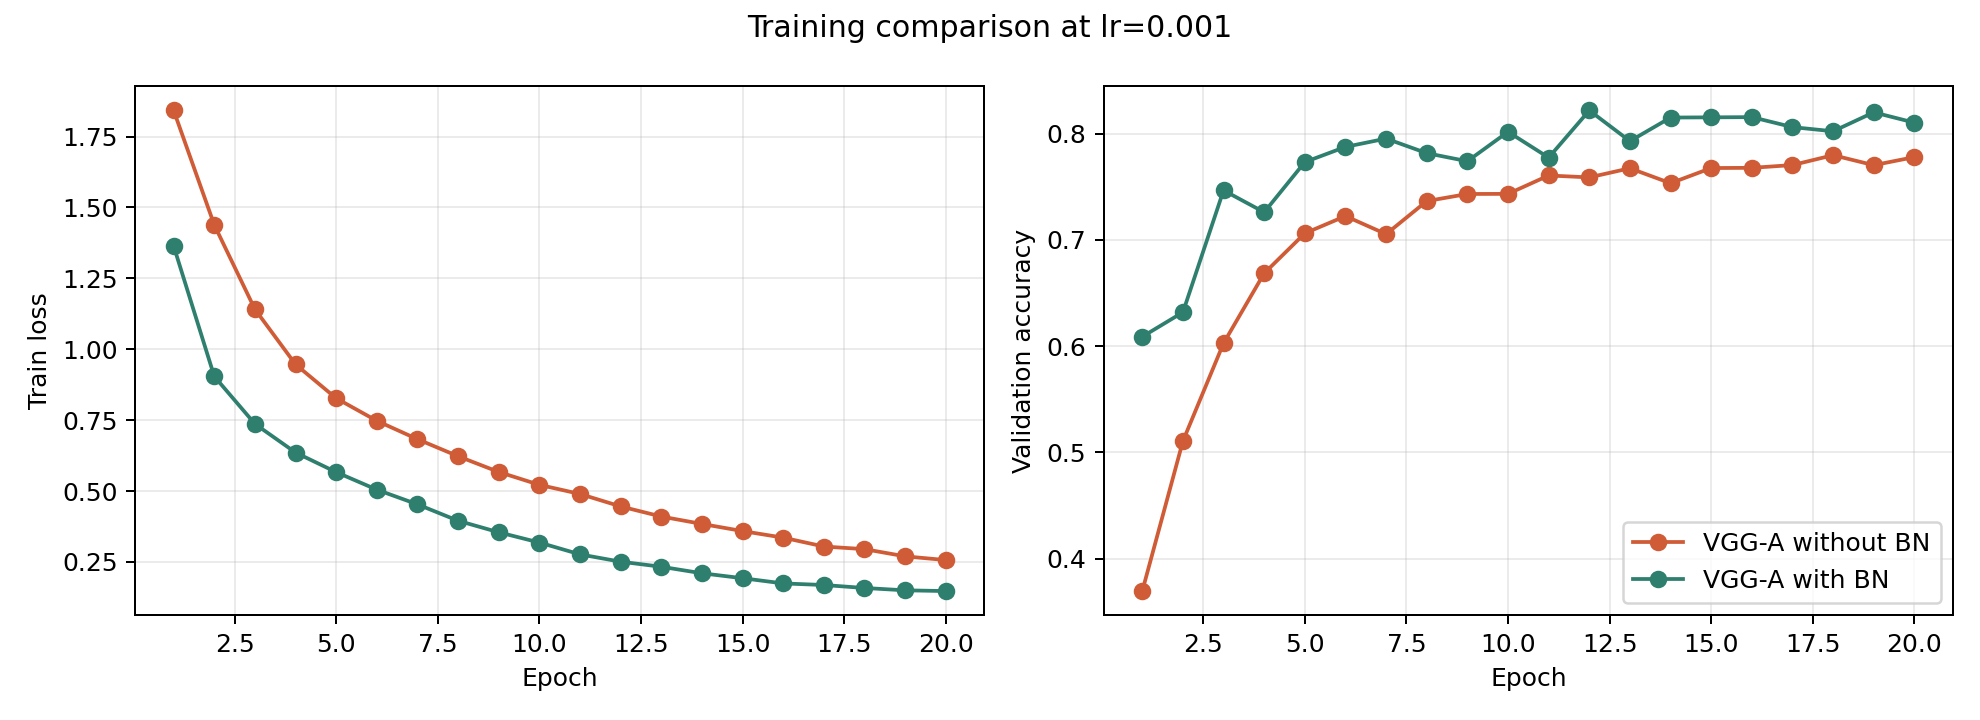
\includegraphics[width=0.92\linewidth]{../Batch_Normalization/results/figures/training_curves_first_lr.png}
  \caption{学习率 $10^{-3}$ 下 VGG-A 与 VGG-A-BN 的训练曲线。BN 模型收敛更快，并达到更高验证准确率。}
  \label{fig:bn_training_curves}
\end{figure}

\subsection{Loss landscape 包络}

项目说明建议通过多学习率训练曲线构造 loss landscape 包络。具体做法是选择多个学习率训练模型，并在同一训练 step 上统计所有模型训练 loss 的最大值与最小值：
\[
\mathrm{max\_curve}(t)=\max_i L_i(t),
\qquad
\mathrm{min\_curve}(t)=\min_i L_i(t).
\]
两条曲线之间的区域反映了训练 loss 对学习率变化的敏感性。包络越宽，说明同一训练 step 下不同学习率导致的 loss 差异越大；包络越窄，则说明优化过程对步长更鲁棒。

\begin{figure}[H]
  \centering
  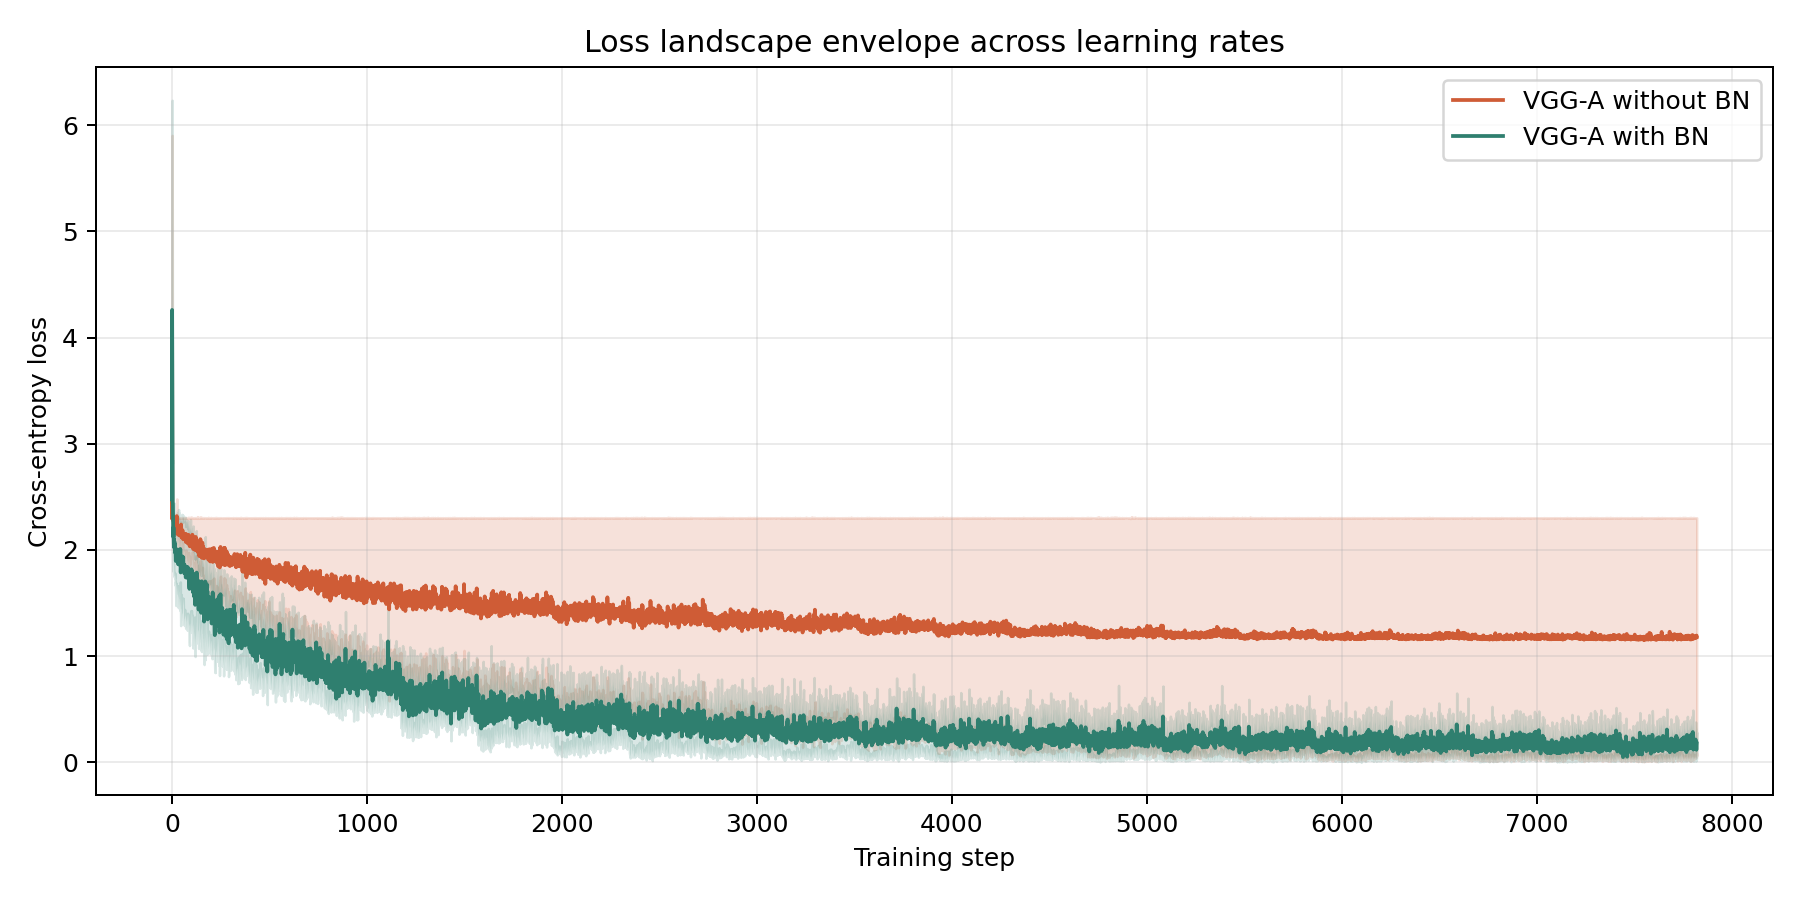
\includegraphics[width=0.9\linewidth]{../Batch_Normalization/results/figures/loss_landscape_envelope.png}
  \caption{VGG-A 与 VGG-A-BN 的跨学习率 loss 包络。BN 显著缩小不同学习率训练曲线之间的 loss 波动范围。}
  \label{fig:bn_loss_envelope}
\end{figure}

对包络宽度进行统计，结果见表~\ref{tab:bn_landscape_width}。BN 的平均包络宽度为 0.375，而无 BN 为 1.900，约减少 $80.3\%$。中位数宽度也从 2.077 降至 0.355。

\begin{table}[H]
  \centering
  \caption{Loss landscape 包络宽度统计}
  \label{tab:bn_landscape_width}
  \begin{tabular}{ccccc}
    \toprule
    模型 & 平均宽度 & 中位数宽度 & 90 分位宽度 & 最大宽度 \\
    \midrule
    VGG-A & 1.900 & 2.077 & 2.262 & 3.603 \\
    VGG-A-BN & $\mathbf{0.375}$ & $\mathbf{0.355}$ & $\mathbf{0.564}$ & 3.948 \\
    \bottomrule
  \end{tabular}
\end{table}

BN 的最大宽度略高，主要来自训练初期个别 batch 的尖峰；但平均值、中位数和 90 分位数均显著更低。因此更合理的结论是：BN 让绝大多数训练过程中的 loss variation 变小，从而使优化路径更稳定。

\subsection{学习率敏感性}

为了系统观察 BN 是否扩大可用学习率范围，我进一步运行学习率 sweep，学习率列表为：
\[
5\times10^{-5},\ 10^{-4},\ 5\times10^{-4},\ 10^{-3},\ 2\times10^{-3},\ 3\times10^{-3},\ 5\times10^{-3}.
\]
结果见表~\ref{tab:bn_lr_sweep}。

\begin{table}[H]
  \centering
  \caption{学习率敏感性实验结果}
  \label{tab:bn_lr_sweep}
  \begin{tabular}{cccc}
    \toprule
    学习率 & VGG-A best acc & VGG-A-BN best acc & BN 提升 \\
    \midrule
    $5\times10^{-5}$ & $75.09\%$ & $70.58\%$ & $-4.51$ pp \\
    $10^{-4}$ & $76.84\%$ & $74.71\%$ & $-2.13$ pp \\
    $5\times10^{-4}$ & $79.25\%$ & $81.82\%$ & $+2.57$ pp \\
    $10^{-3}$ & $77.97\%$ & $\mathbf{82.18\%}$ & $+4.21$ pp \\
    $2\times10^{-3}$ & $10.00\%$ & $81.36\%$ & $+71.36$ pp \\
    $3\times10^{-3}$ & $10.00\%$ & $79.46\%$ & $+69.46$ pp \\
    $5\times10^{-3}$ & $65.49\%$ & $75.00\%$ & $+9.51$ pp \\
    \bottomrule
  \end{tabular}
\end{table}

\begin{figure}[H]
  \centering
  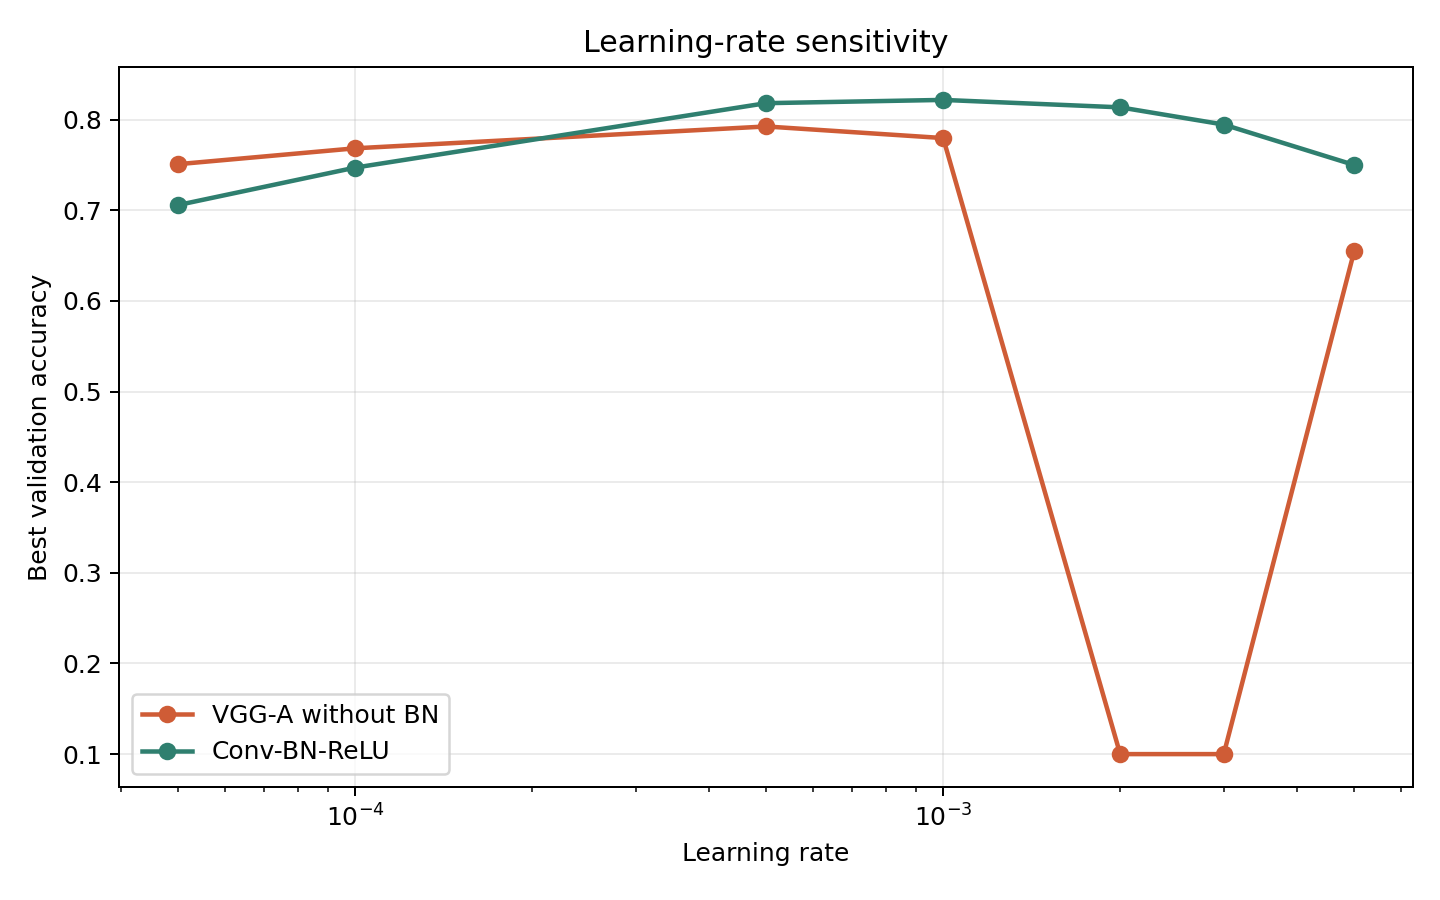
\includegraphics[width=0.78\linewidth]{../Batch_Normalization/Enhanced/results/figures/lr_sensitivity.png}
  \caption{学习率敏感性曲线。BN 在较大学习率下仍能保持有效训练，而无 BN 模型在 $2\times10^{-3}$ 和 $3\times10^{-3}$ 下崩溃。}
  \label{fig:bn_lr_sensitivity}
\end{figure}

该实验说明，BN 的收益具有条件性。小学习率下，普通 VGG-A 已经可以稳定下降，BN 不一定更优；学习率增大后，无 BN 模型更容易进入不稳定区域，而 BN 仍能保持较高准确率。因此 BN 的核心价值可以概括为扩大可用学习率区间，提高训练对超参数选择的鲁棒性。

\subsection{梯度预测性}

项目说明还要求分析 gradient predictiveness，即当前梯度对附近 loss landscape 的预测能力。为此，我记录相邻 step 的梯度变化。设第 $t$ 步梯度为 $g_t$，参数为 $w_t$，定义：
\[
\Delta_g(t)=\|g_t-g_{t-1}\|_2,
\]
\[
r_g(t)=\frac{\|g_t-g_{t-1}\|_2}{\|g_{t-1}\|_2+\epsilon},
\]
\[
c_g(t)=\frac{g_t^\top g_{t-1}}{\|g_t\|_2\|g_{t-1}\|_2+\epsilon},
\]
以及距离归一化的梯度变化：
\[
D_g(t)=\frac{\|g_t-g_{t-1}\|_2}{\|w_t-w_{t-1}\|_2+\epsilon}.
\]
其中 $r_g$ 越小、$c_g$ 越大，通常表示相邻 step 的梯度方向更一致，局部线性近似更有预测性。

\begin{table}[H]
  \centering
  \caption{代表性学习率下的梯度预测性统计}
  \label{tab:bn_gradient_predictiveness}
  \begin{tabular}{cccccc}
    \toprule
    学习率 & 模型 & Best acc & 平均相对梯度变化 & 平均梯度余弦 & 最大 $D_g$ \\
    \midrule
    $10^{-3}$ & VGG-A & $77.97\%$ & 1.338 & 0.170 & 79.59 \\
    $10^{-3}$ & VGG-A-BN & $82.18\%$ & 1.368 & 0.144 & $\mathbf{49.46}$ \\
    $2\times10^{-3}$ & VGG-A & $10.00\%$ & 1.490 & 0.003 & 21.62 \\
    $2\times10^{-3}$ & VGG-A-BN & $81.36\%$ & 1.353 & 0.154 & 29.59 \\
    $3\times10^{-3}$ & VGG-A & $10.00\%$ & 1.642 & 0.005 & 33.70 \\
    $3\times10^{-3}$ & VGG-A-BN & $79.46\%$ & 1.342 & 0.149 & $\mathbf{18.74}$ \\
    \bottomrule
  \end{tabular}
\end{table}

梯度指标需要谨慎解释。比如在 $2\times10^{-3}$ 下，无 BN 模型已经退化到随机猜测附近，此时某些梯度范数或梯度变化可能较小，但这并不代表优化稳定，而是模型没有进入有效学习状态。更有意义的是结合准确率观察：在较大学习率下，无 BN 的梯度方向连续性几乎消失，平均梯度余弦接近 0；BN 则仍保持可训练状态，并取得 $80\%$ 左右准确率。

\begin{figure}[H]
  \centering
  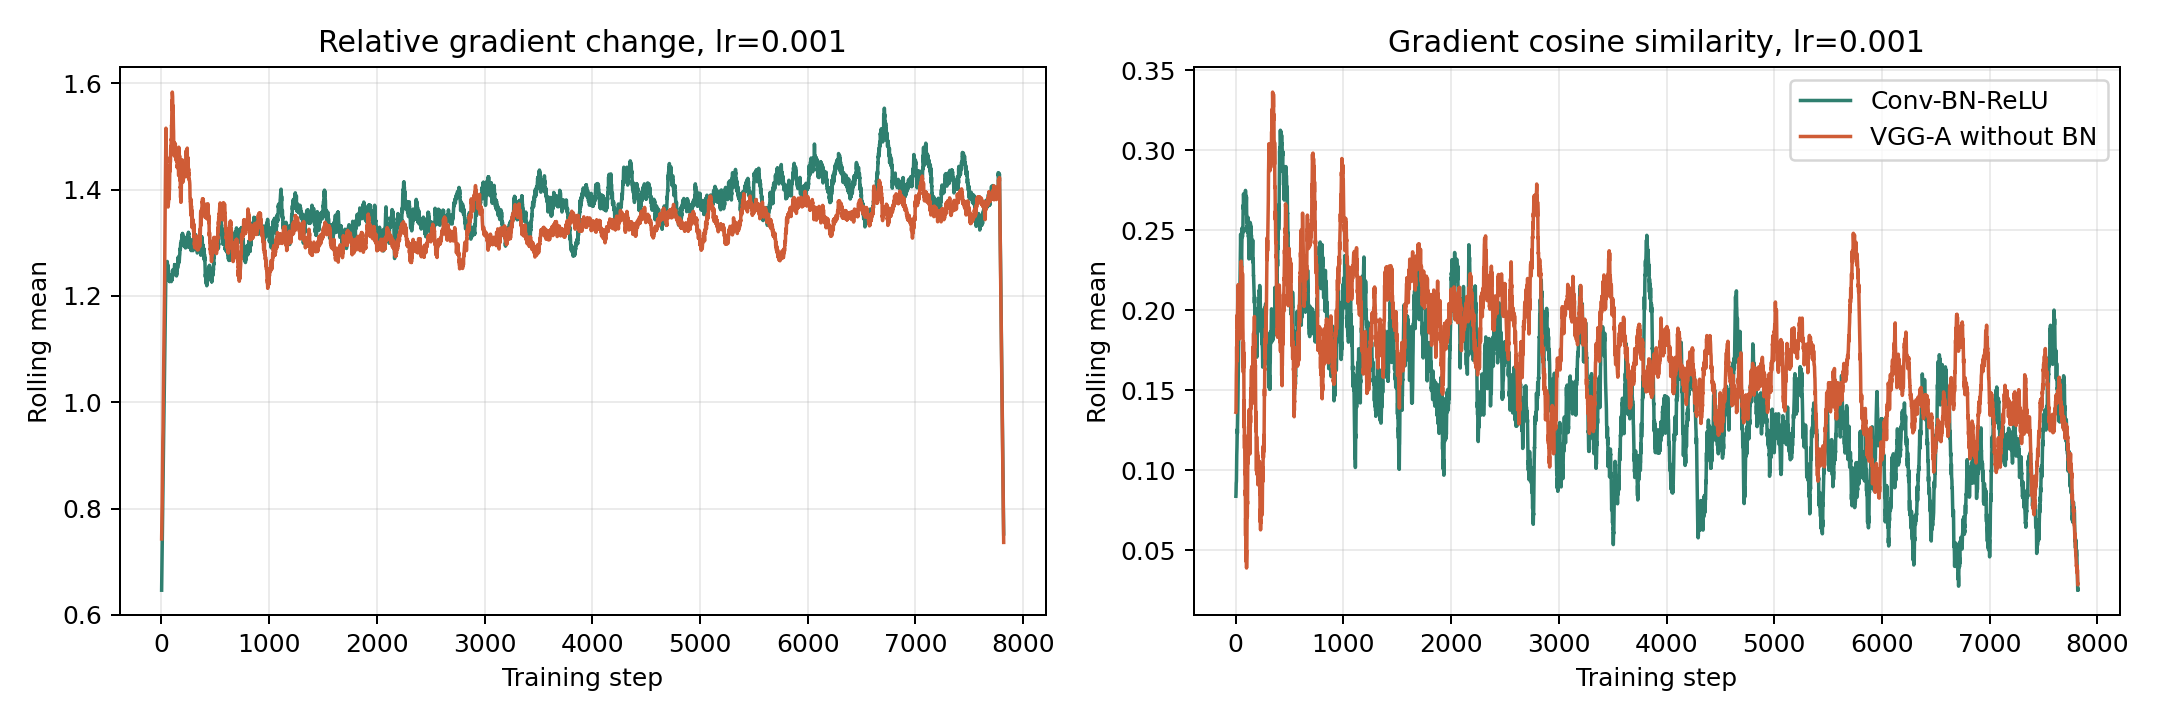
\includegraphics[width=0.9\linewidth]{../Batch_Normalization/Enhanced/results/figures/gradient_predictiveness.png}
  \caption{梯度预测性可视化。梯度变化指标必须与最终准确率共同解释，避免把训练失败后的低梯度误读为稳定优化。}
  \label{fig:bn_gradient_predictiveness}
\end{figure}

\subsection{进一步可视化：二维 loss surface 与激活分布}

除了项目要求的 loss 包络，我还使用已训练 checkpoint 在参数空间中选取两个 filter-normalized random directions，绘制局部二维 loss surface：
\[
L(w+\alpha d_1+\beta d_2).
\]
该图是高维参数空间的二维切片，不代表完整 loss landscape，但可以直观展示 checkpoint 附近的曲面形态。

\begin{figure}[H]
  \centering
  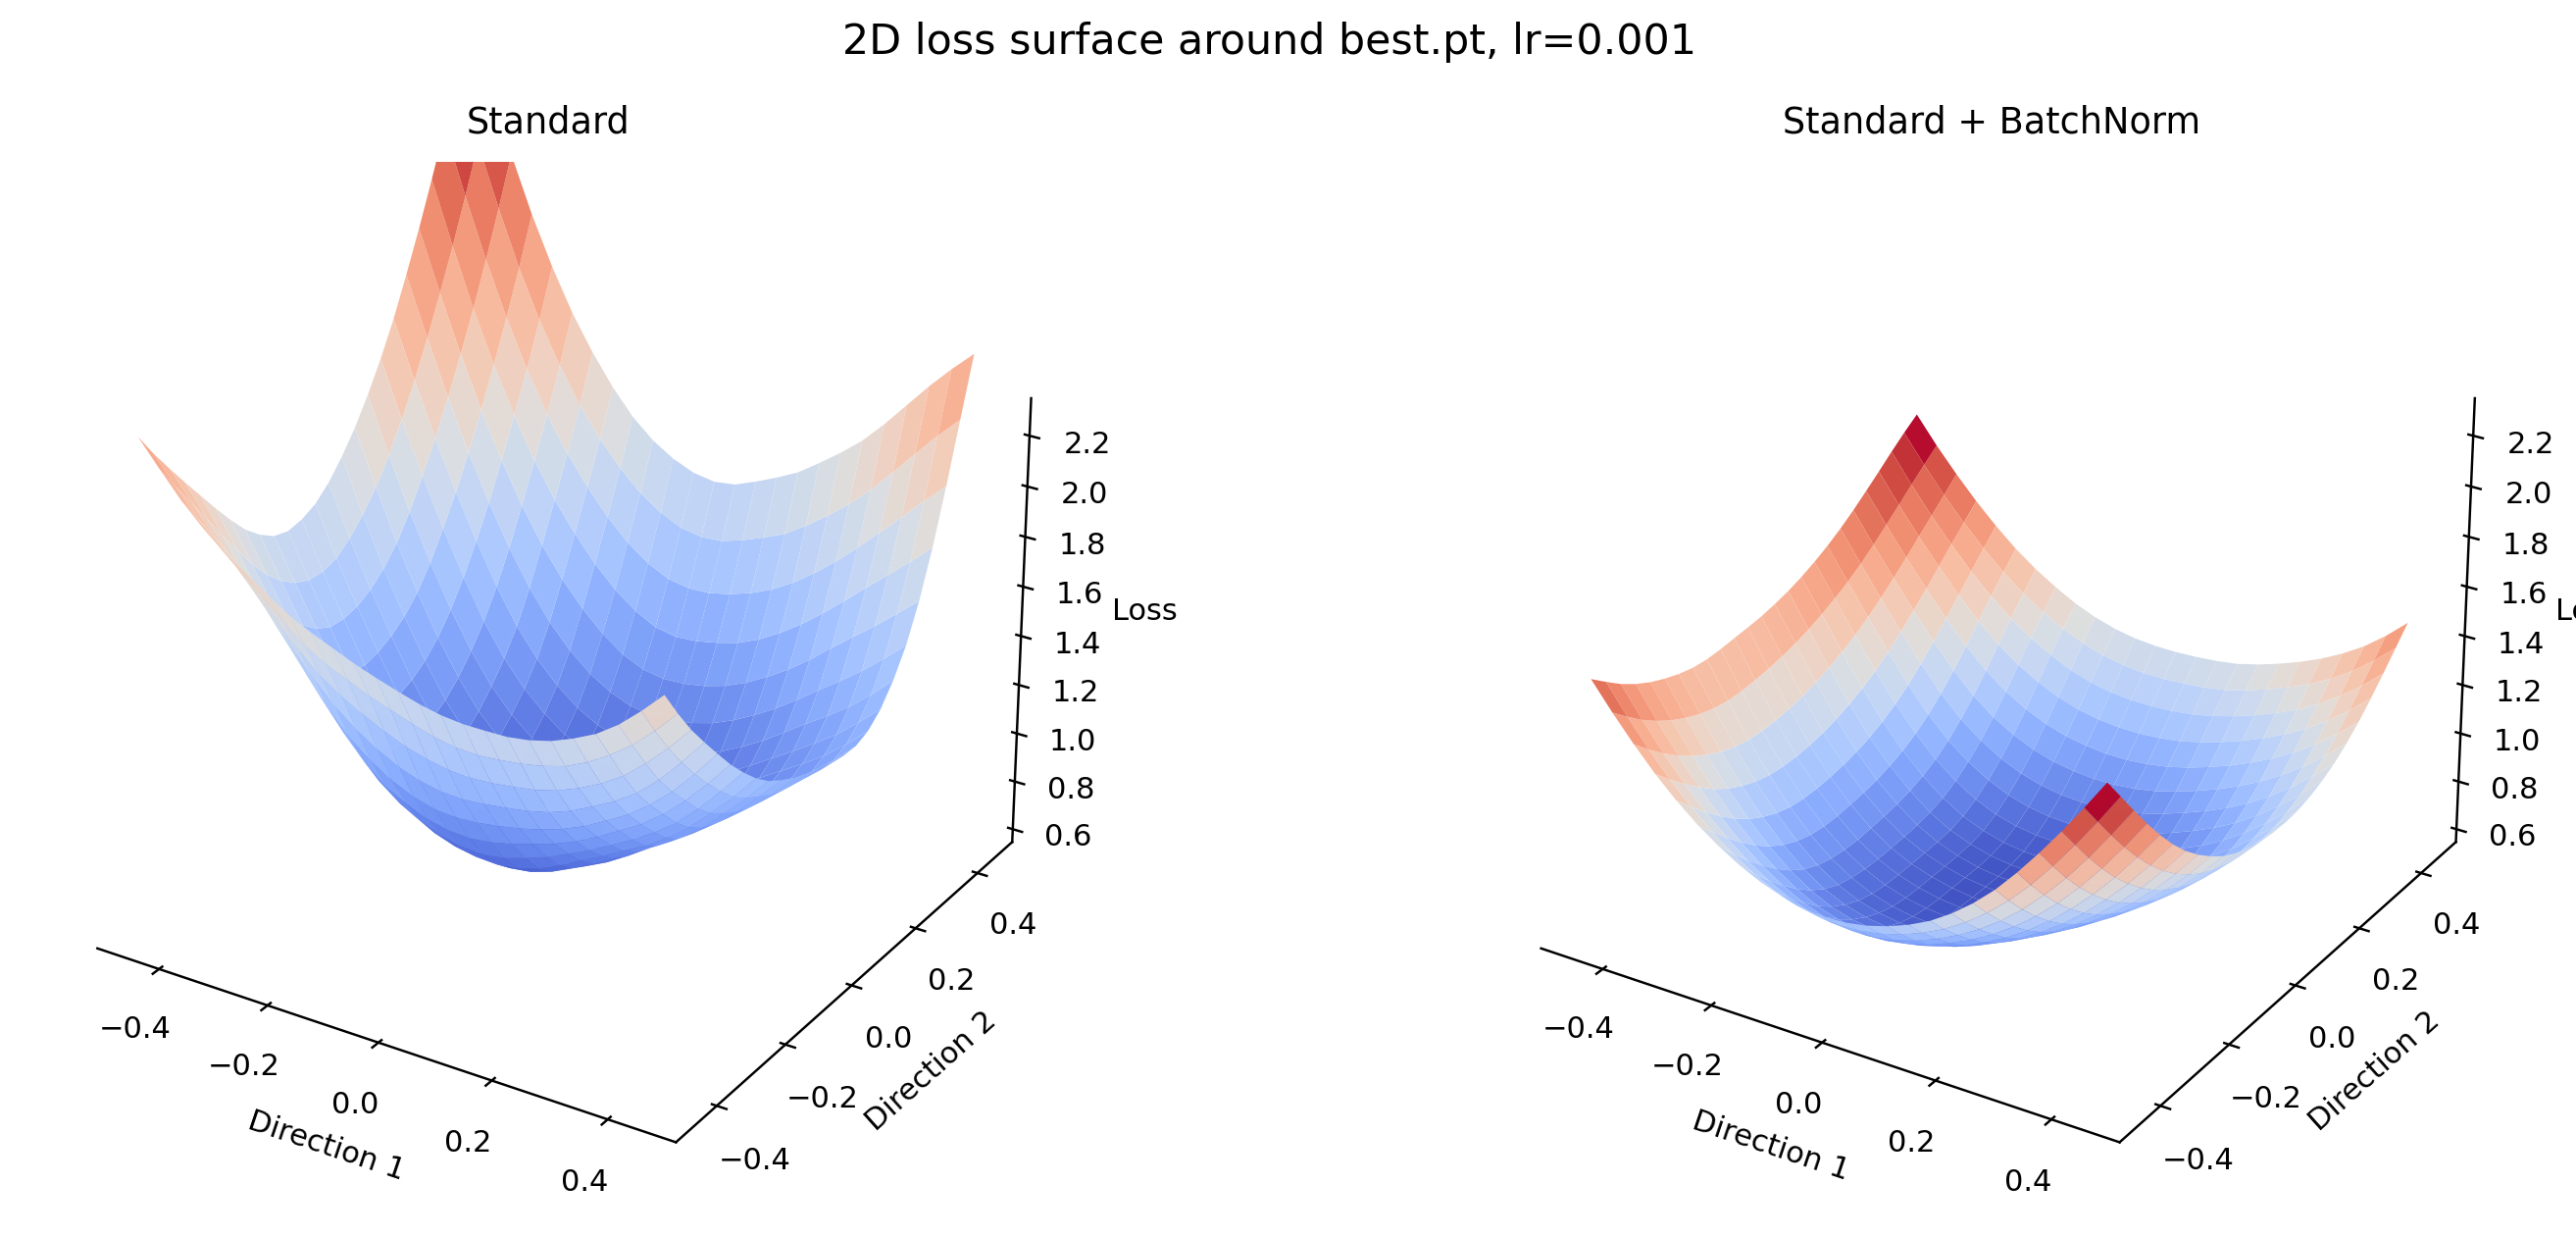
\includegraphics[width=0.9\linewidth]{../Batch_Normalization/Visual/figures/loss_surface_3d_no_bn_vs_bn.png}
  \caption{VGG-A 与 VGG-A-BN 的局部二维 loss surface。该图作为直观补充，严谨结论仍以跨学习率包络和统计指标为主。}
  \label{fig:bn_loss_surface}
\end{figure}

为了观察 BN 对中间表征的影响，我还采集若干卷积层附近的激活分布。对无 BN 模型采集卷积输出；对 BN 模型采集对应 BatchNorm 层输出。

\begin{figure}[H]
  \centering
  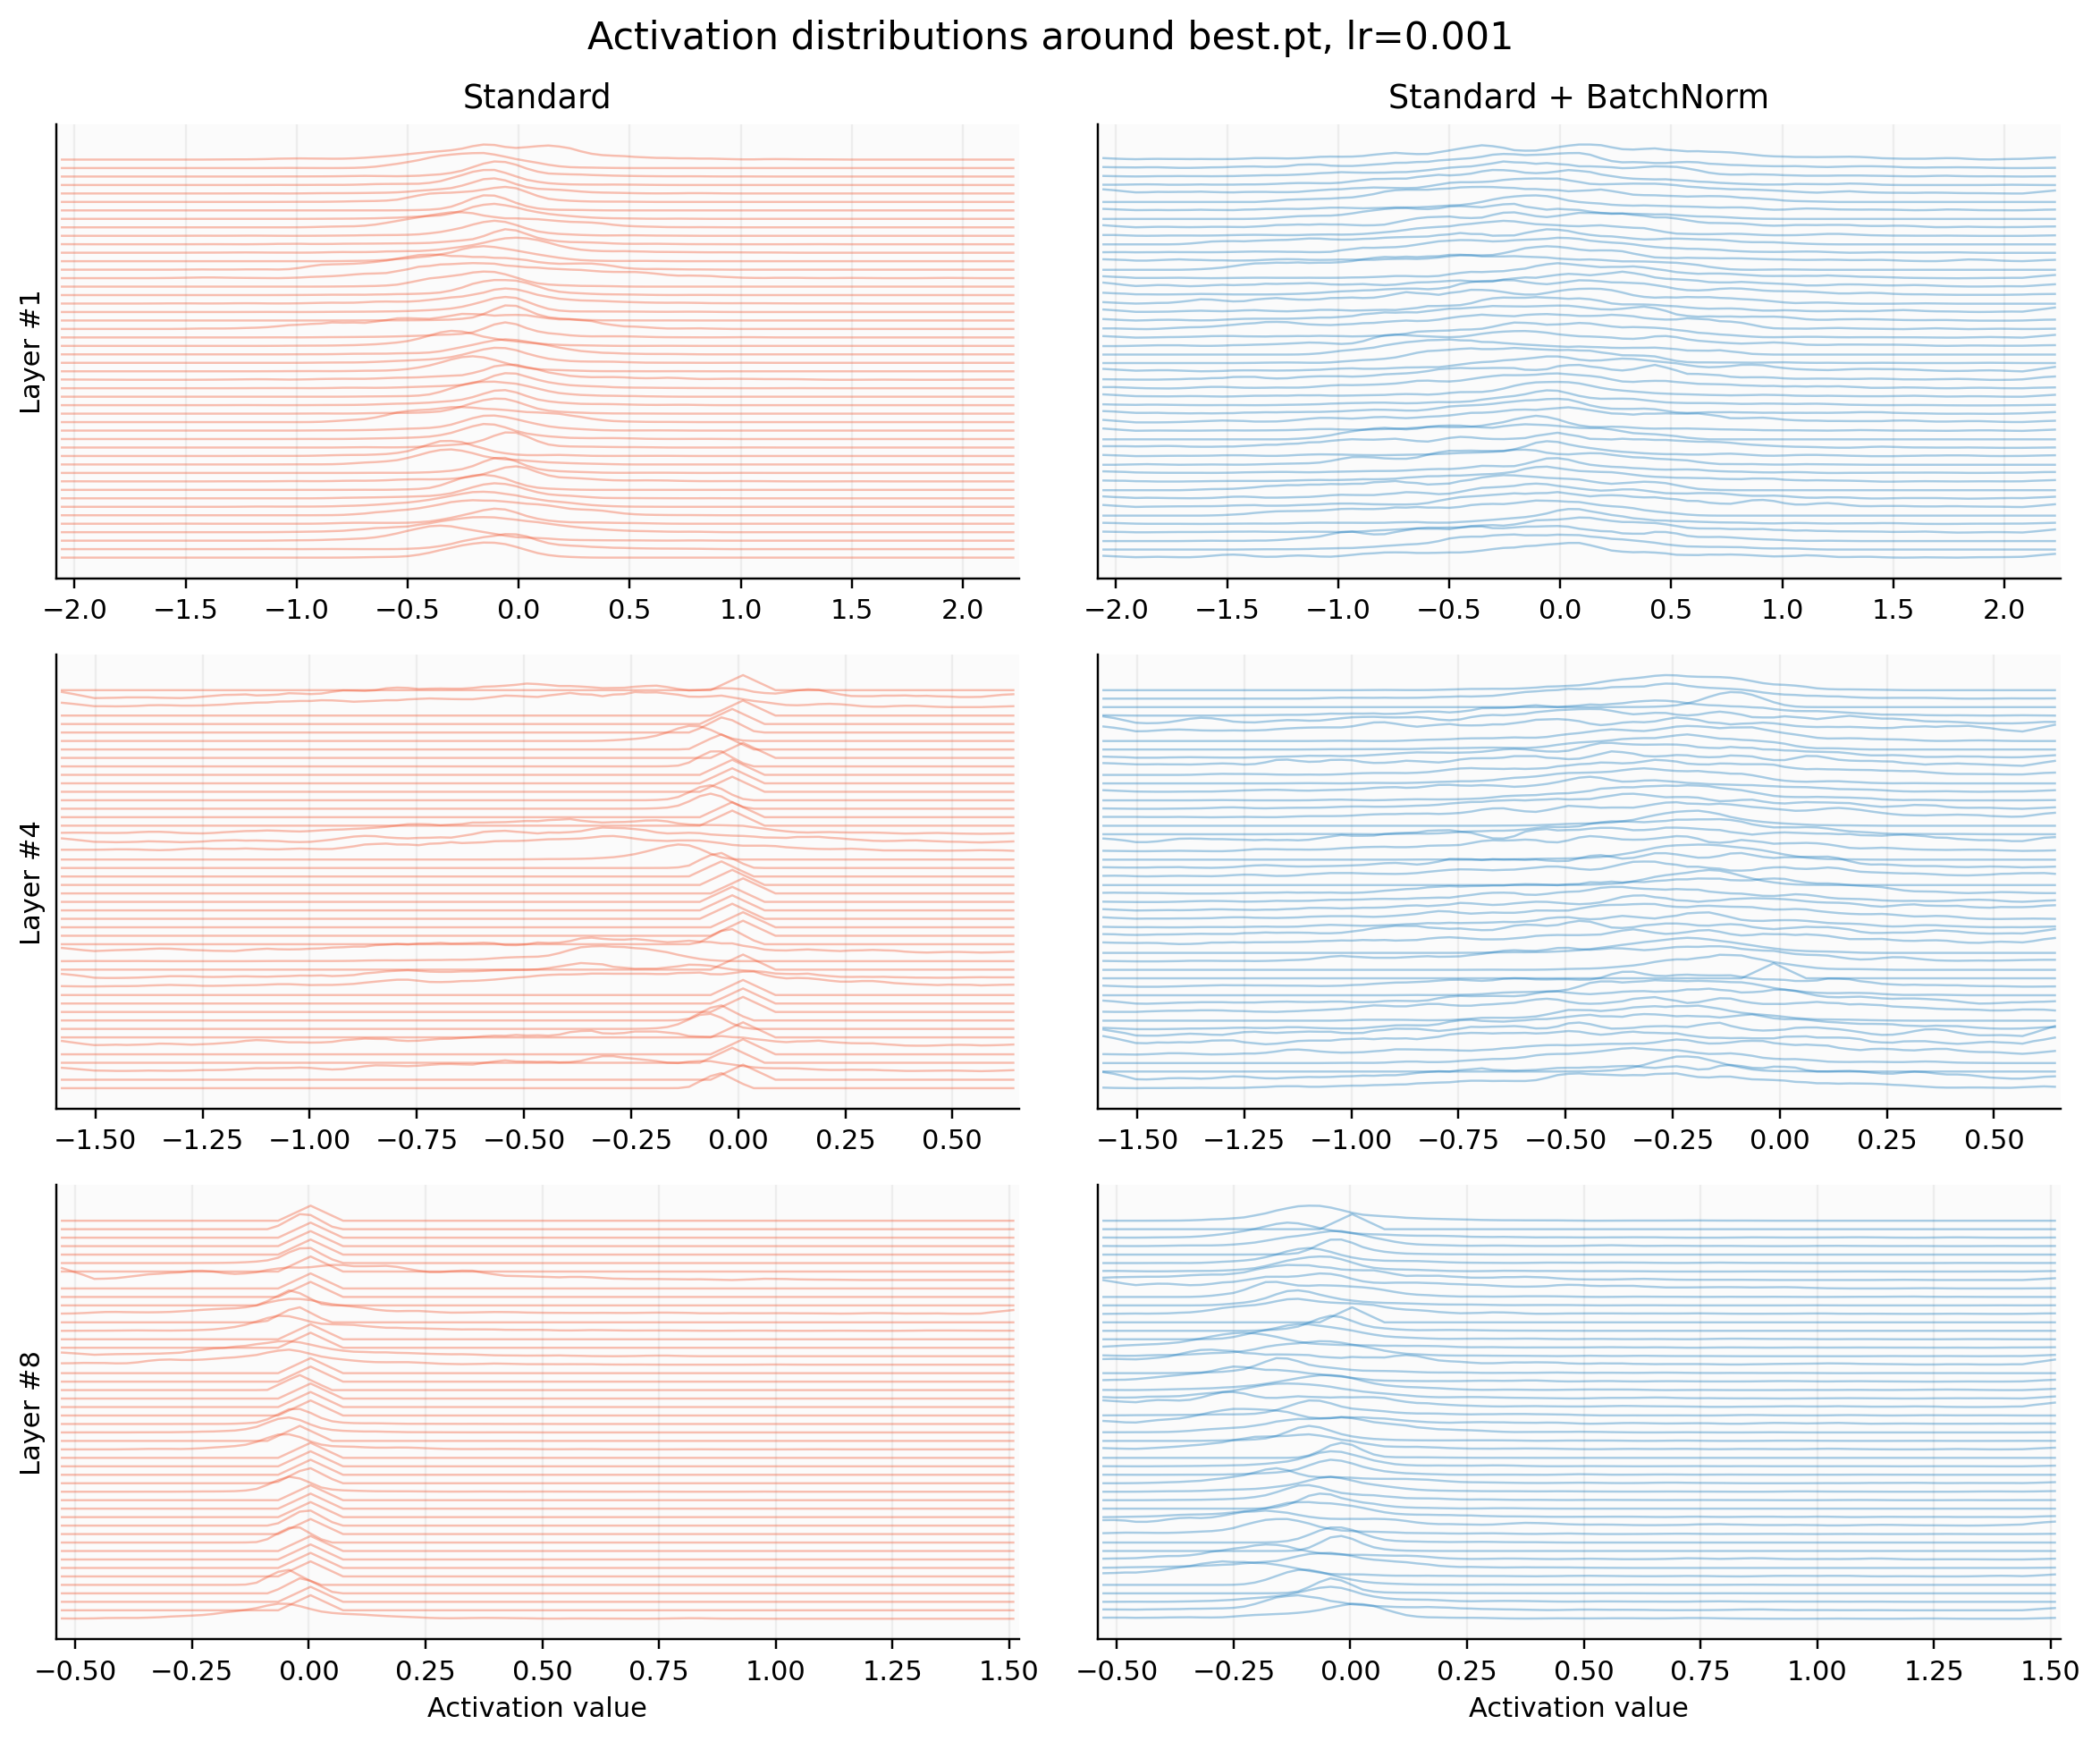
\includegraphics[width=0.92\linewidth]{../Batch_Normalization/Visual/figures/activation_distribution_ridgeline.png}
  \caption{VGG-A 与 VGG-A-BN 的激活分布 ridgeline。BN 引入通道级重参数化，使中间表征尺度受到更直接的控制。}
  \label{fig:bn_activation_distribution}
\end{figure}

需要注意的是，训练完成后的 BN 输出并不一定严格保持零均值单位方差，因为 BN 后还有可学习的 $\gamma,\beta$，并且测试时使用 running statistics。因此激活图不能被简单解释为“BN 后所有分布都更窄”。更合理的理解是：BN 在训练过程中提供了受控的通道级重参数化，使每层输入分布不完全由前层权重漂移决定，从而改善梯度下降的有效性。

\subsection{BN 部分结论}

综合基础实验、loss 包络、学习率 sweep 和梯度预测性分析，可以得到以下结论：

\begin{enumerate}
  \item BN 在中等和较大学习率下显著提升 VGG-A 的训练稳定性。$10^{-3}$ 下准确率提升 4.21 个百分点；$2\times10^{-3}$ 下无 BN 崩溃，BN 仍达到 $81.36\%$。
  \item BN 显著缩小跨学习率 loss 包络。平均包络宽度从 1.900 降至 0.375，说明训练 loss 对学习率变化更不敏感。
  \item BN 扩大了可用学习率范围。无 BN 在 $2\times10^{-3}$ 和 $3\times10^{-3}$ 下停留在随机猜测，而 BN 仍保持约 $80\%$ 的准确率。
  \item 梯度预测性实验说明，BN 的作用不能只看单个梯度范数，而应结合训练是否成功。BN 的核心价值在于让较大学习率下的梯度更新仍然有效。
\end{enumerate}

这些结果与 Santurkar 等人提出的观点一致：BN 的关键贡献并不仅仅是减少 internal covariate shift，而是通过重参数化使实际训练路径上的优化问题更加平滑，从而提高梯度下降类方法的稳定性。

\subsection{项目总体结论}

本项目的最终提交结果可以概括为两点。首先，在 CIFAR-10 分类任务中，最终 SE-DenseNet-BC-190-24 以约 9.98M 参数达到 $97.15\%$ 测试准确率和 $2.85\%$ 测试错误率，相比 DenseNet-BC、WideResNet 和早期 SE-DenseNet-BC-190-40 候选模型均有进一步提升。该结果来自结构设计、容量选择、GELU 激活、SGD 训练、CutMix/AutoAugment/Cutout、label smoothing 和 EMA 的组合，而不是单一技巧的孤立作用。其次，在 Batch Normalization 实验中，VGG-A-BN 在中等和较大学习率下明显优于 VGG-A；跨学习率 loss 包络宽度从 1.900 降至 0.375，说明 BN 通过改善优化稳定性扩大了可用学习率范围。两部分实验共同说明，深度网络性能不仅取决于模型容量，也高度依赖优化路径、正则化方式和训练动态的稳定性。

\appendix
\section{提交链接与复现说明}

\subsection{代码、权重与数据集链接}

GitHub 代码仓库：
\begin{center}
\url{https://github.com/KouseiAimer/Network-and-Deep-Learning-Second-Project}
\end{center}

ModelScope 模型权重仓库：
\begin{center}
\url{https://modelscope.cn/models/KouseiAimer/Network-and-Deep-Learning-Second-Project}
\end{center}

CIFAR-10 官方数据集：
\begin{center}
\url{https://www.cs.toronto.edu/~kriz/cifar.html}
\end{center}

ModelScope 中的权重路径与 GitHub 仓库中的相对路径保持一致。最终模型权重为：
\begin{verbatim}
Ablation/results/final/best_from_ablation/weights/best.pt
Ablation/results/final/best_from_ablation/weights/last.pt
\end{verbatim}

\subsection{最终模型验证命令}

在项目根目录运行：
\begin{verbatim}
conda activate dl
python quick_check.py --num-workers 0
\end{verbatim}

期望输出：
\begin{verbatim}
test_accuracy : 97.15%
test_error    : 2.85%
correct/total : 9715/10000
\end{verbatim}

\subsection{主要代码入口}

第一部分消融与最终训练：
\begin{verbatim}
python Ablation/ablation.py --epochs 50 --amp
python Ablation/visual_ablation.py
python Ablation/final.py --epochs 300 --amp
python Ablation/visual_final.py
\end{verbatim}

第二部分 BN 基础实验与可视化：
\begin{verbatim}
python Batch_Normalization/run_bn_experiments.py --epochs 20 \
  --learning-rates 1e-3 2e-3 5e-4 1e-4 --batch-size 128

python Batch_Normalization/Enhanced/run_enhanced_experiments.py \
  --suite lr_sweep --epochs 20

python Batch_Normalization/Visual/visualize_bn.py --mode all
\end{verbatim}

\begin{thebibliography}{9}
\bibitem{krizhevsky2009}
Alex Krizhevsky.
\newblock Learning Multiple Layers of Features from Tiny Images.
\newblock Technical report, 2009.

\bibitem{ioffe2015}
Sergey Ioffe and Christian Szegedy.
\newblock Batch Normalization: Accelerating Deep Network Training by Reducing Internal Covariate Shift.
\newblock ICML, 2015.

\bibitem{santurkar2018}
Shibani Santurkar, Dimitris Tsipras, Andrew Ilyas, and Aleksander Madry.
\newblock How Does Batch Normalization Help Optimization?
\newblock NeurIPS, 2018.

\bibitem{huang2017}
Gao Huang, Zhuang Liu, Laurens van der Maaten, and Kilian Q. Weinberger.
\newblock Densely Connected Convolutional Networks.
\newblock CVPR, 2017.

\bibitem{hu2018}
Jie Hu, Li Shen, and Gang Sun.
\newblock Squeeze-and-Excitation Networks.
\newblock CVPR, 2018.
\end{thebibliography}

\end{document}
